%%%%%%%%%%%%%%%%%%%%
%%%%%  Methods %%%%%
%%%%%%%%%%%%%%%%%%%%

\chapter{Materials and Methods} \label{Ch:MasterialsAndMethods}
In this chapter, the materials and methods at the core of this thesis are discussed. Starting with a section on efficient image registration using neural networks, the problem of efficient registration is explained and the network architectures of \emph{Fourier-Net} and \emph{Fourier-Net+} are presented in detail. After this, the pipeline used for the motion-compensated reconstruction is explained followed by the datasets used in this thesis. Lastly, the experiments conducted in this thesis are described. These include ablation studies, parameter tests, tests for registration performance and the evaluation of a motion-compensated reconstruction pipeline for cardiac MR data.

\section{Efficient Registration using Neural Networks} \label{Sec:NetworkArchitecture}
As a starting point, \emph{Fourier-Net}~\cite{Fourier-Net} and its successor \emph{Fourier-Net+}~\cite{Fourier-Net+} were used. These networks, which are explained in the following pages, enable fast and accurate registration while needing less resources compared to similar approaches. These attributes are very beneficial for a potential application like motion correction because the current networks, e.g. \emph{LAPNet}, are usually supervised and require large computational resources.

\subsection{Problem Formulation} \label{SubSec:ProblemFormulation}
While there are many different traditional iterative algorithms that are proven to work~\cite{DARTEL,Vercauteren2009,NiftiReg,LAP,FLASH} these all suffer from heavy computational requirements and long registration times~\cite{Chen2023} as discussed previously in section~\ref{Sec:RelatedWork}. While neural networks like~\cite{LAPNet,DeepFlash} could be trained in a supervised manner using these conventional algorithms as a basis to alleviate the time problems~\cite{Chen2020}, these were still very memory intensive as well as being unwieldy to train~\cite{Zou2022}. While unsupervised networks like~\cite{Voxelmorph,IC-Net,SYM-Net} could circumvent the latter problem, memory efficiency remained a difficult problem. All of these networks and algorithms predict a dense displacement, some even use complex values which essentially kills their performance. However, a new type of architecture has recently been proposed~\cite{Fourier-Net,Fourier-Net+} that is far more efficient due to predicting only a band-limited displacement, without the need for complex values, while promising similar performance. These networks will be discussed in the next sections.

\subsection{Fourier-Net}	\label{SubSec:Fourier-Net}
\emph{Fourier-Net} is a new unsupervised approach that aims to learn a low-dimensional representation of the displacement field in a band-limited Fourier domain instead of the full field in the spatial domain. This band-limited representation is then decoded by a model-driven decoder to the dense, full-resolution displacement field in the spatial domain. The zero-padding is necessary to keep the spatial resolution in image space without adding any further information. This band-limiting allows for fewer parameters and computational operations, resulting in faster inference speeds~\cite{Fourier-Net}. The architecture is based on the U-Net, like many deep registration approaches, but replaces the expanding path with a parameter-free model-driven decoder o save memory as mentioned before. The encoder of \emph{Fourier-Net} consists of a CNN, which takes two images (fixed and moving) as inputs. The output is a displacement field that is then converted from the spatial domain into the Fourier domain via an discrete Fourier transformation (DFT). From there, this band-limiting representation 
%of the displacement field 
is padded with zeros to the full resolution of the original displacement field. The field is then recovered by using the inverse DFT (iDFT) to convert it back into the spatial domain. This displacement field is then used to warp the moving image into the fixed image. Additionally, squaring and scaling layers~\cite{Dalca2018} can be added before warping the image in order to encourage a diffeomorphism in final deformation. 

\begin{figure}[h] %tpb
	\centering
	\graphicspath{{images/}{\main/images/}}
	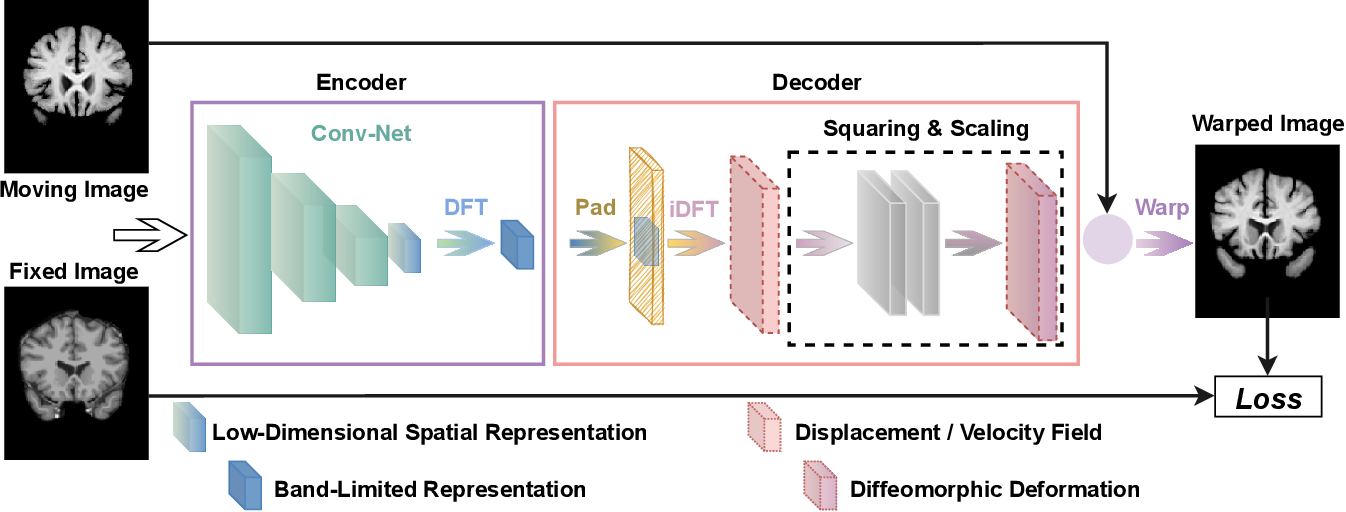
\includegraphics[width=\linewidth]{ArchitectureFourier-Net.png} 
	\caption{Architecture of \emph{Fourier-Net} taken from~\cite{Fourier-Net}. The encoder takes two images as an input and produces a band-limited displacement which is then padded and transformed to image space in the decoder. This output is the full-resolution displacement which is then used to warp the moving image for loss calculation based on its similarity to the fixed image.}
	\label{fig:Fourier-Net}
\end{figure}

\subsubsection{Encoder}	\label{SubSubSec:Encoder}
The encoder of \emph{Fourier-Net} consists of a CNN that generates the displacement field between the two inputs followed by a DFT layer that produces a band-limited representation of the full displacement field. The fully convolutional neural network (FCN) from \emph{SYMNet}~\cite{SYM-Net} was modified to function as the CNN of the encoder. Its (original) architecture (see Figure~\ref{fig:SYMNet}) is again based on the U-Net with a contracting and expanding path. The FCN concatenates the inputs images $X$ and $Y$ as a single 2-channel input and estimates two dense, non-linear displacement fields $\phi_{XY}$ and $\phi_{YX}$, however we only need the displacement field for the moving image, denoted as $\mathbb{S}_\phi$, since we are not interested in transforming the fixed image. This is actually a low dimensional representation because \emph{Fourier-Net} does not utilize the last two levels of the FCNs expanding path that would be needed to reconstruct the actual full-resolution displacement field $\phi$.\\
For each level in the contracting path of the FCN, two successive convolution layers are applied, which contain one $3 \times 3 \times 3$ convolution layer with a stride of 1, followed by a $3 \times 3 \times 3$ convolution layer with a stride of 2 to further compute the high-level features between the input images as well as downsampling the features by half until the lowest level of the network is reached. For each level in the expanding path of the FCN, the feature maps from the contracting path are concatenated through skip connections and apply $3 \times 3 \times 3$ convolution with a stride of 1 and $2 \times 2 \times 2$ de-convolution layer for upsampling the feature maps to twice of its size. At the end of the expanding path, two $5 \times 5 \times 5$ convolution layers with a stride of 1 are appended to the last convolution layer and generate the displacement fields $\theta_{XY}$ and $\theta_{YX}$~\cite{SYM-Net}. Each convolution layer in the FCN is followed by a rectified linear unit (ReLU) activation, except for the output convolution layer that does not have an activation function because \emph{Fourier-Net} only uses the first two levels of the expanding path, thus leading the FCN to generate a low dimensional representation $\mathbb{S}_\phi$ of the full-resolution displacement field $\phi$.\\
%, where a SoftSign activation function is used~\cite{SYM-Net}:
%\begin{equation}
%	\text{SoftSign}(x) = \frac{x}{1 + |x|} .
%\end{equation}
As discussed previously, the encoder aims to learn a displacement (or velocity) field in the band-limited Fourier domain. Intuitively, this may require convolutions to be able to handle complex-valued numbers, which can be done by using complex-valued CNNs~\cite{Trabelsi2017}, which are suitable when both input and output are complex values, however these complex-valued operations sacrifice computational efficiency. Other approaches like \emph{DeepFlash}~\cite{DeepFlash} tackle this problem by converting the input images to the Fourier domain and using two individual real-valued CNNs to learn the real and imaginary parts separately. This, however, increases training and inference cost. To bridge the domain gap between real-valued spatial images and complex-valued band-limited displacement fields without increasing complexity, \emph{Fourier-Net} uses a DFT layer after the FCN. This is a simple and effective way to produce complex-valued band-limited displacement fields without the network needing to be able to handle complex values or learn a mapping between the image and frequency domain. The DFT applied to the displacement field $\phi$ can be defined as follows:
\begin{equation} \label{eq:DFT}
	[\mathcal{F}(\phi)]_{k,l} = \sum^{H-1}_{n=0} \sum^{W-1}_{m=0} \phi_{n,m} \cdot \exp \Bigg(i \cdot \bigg(\frac{2 \pi k}{H} \cdot n + \frac{2 \pi l}{W} \cdot m \bigg) \Bigg),
\end{equation}
where $\phi$ has size $H \times W$ with $H$ and $W$ being the spatial dimensions in 2D. $n \in [0,H-1]$ and $m \in [0,W-1]$ are the discrete indices in the spatial domain, and $k \in [0,H-1]$ and $l \in [0,W-1]$ are the discrete indices in the frequency domain with $i$ being the imaginary unit. However, $\phi$ in this equation is actually the low dimensional representation of the displacement field output by the modified FCN, which can be formulated as follows:
\begin{equation} \label{eq:FCN}
	\mathbb{S}_\phi = \text{FCN}(M,F;\Theta),
\end{equation}
with $M$ being the moving and $F$ the fixed image, as well as $\Theta$ representing the parameters of the FCN. Thus, the whole encoder can be defined as:
\begin{equation}\label{eq:encoder}
	\mathbb{B}_\phi = \mathcal{F}(\mathbb{S}_\phi) = \mathcal{F}(\text{FCN}(M,F;\Theta)),
\end{equation}
with the DFT layer $\mathcal{F}$, full-resolution spatial displacement field $\phi$ and the complex band-limited displacement field $\mathbb{B}_\phi$. The low dimensional representation $\mathbb{S}_\phi$ actually contains all the information of the band-limited Fourier coefficients in $\mathbb{B}_\phi$. As such, \emph{Fourier-Net} does not need to learn the coefficients of $\mathbb{B}_\phi$, but instead only the real-valued coefficients in $\mathbb{S}_\phi$, which is the low dimensional spatial representation of the full-resolution spatial displacement field $\phi$, which is then reconstructed by the decoder. 

\begin{figure}[h] %tpb
	\centering
	\graphicspath{{images/}{\main/images/}}
	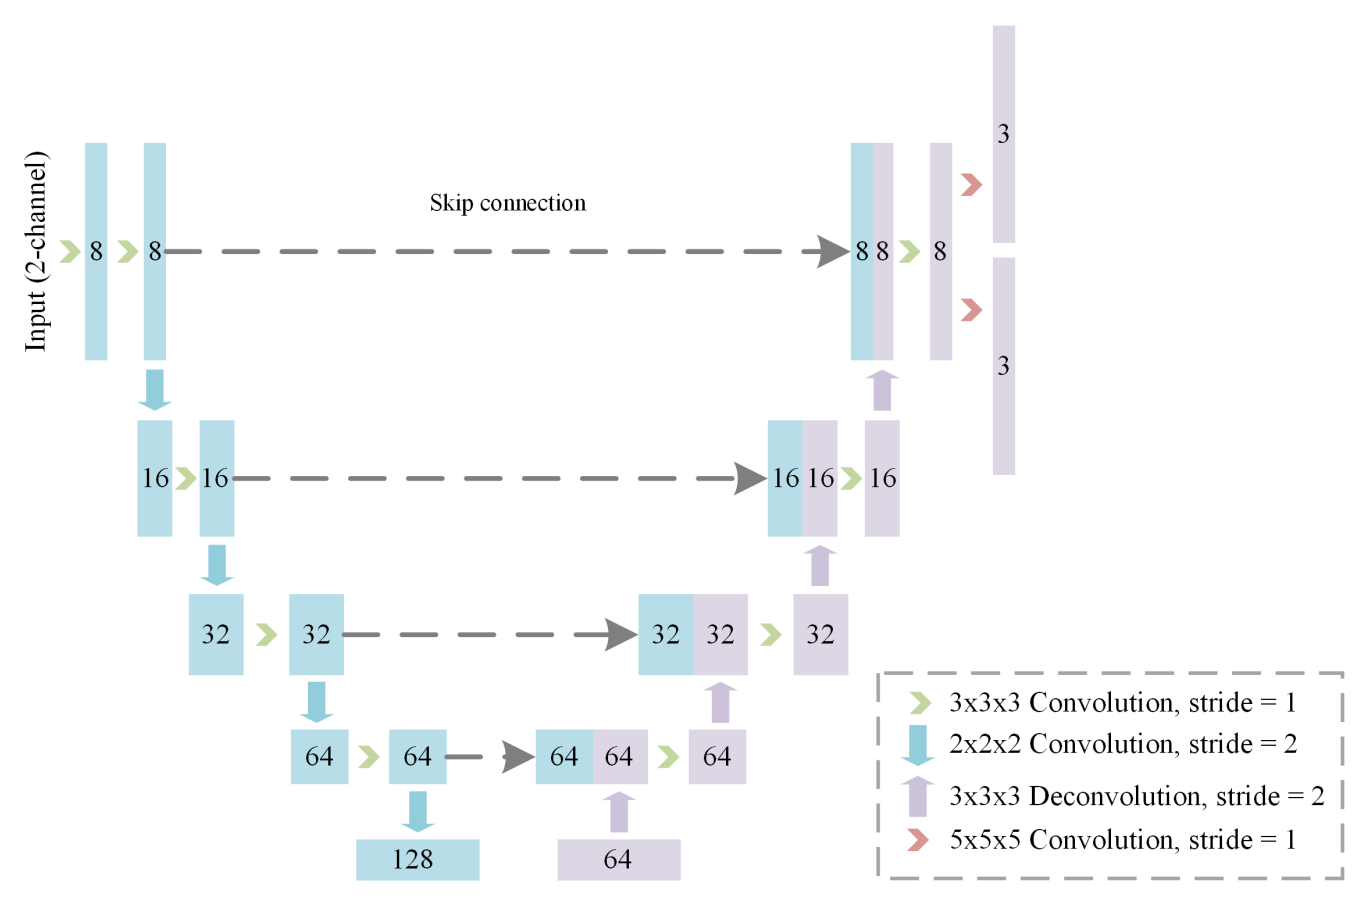
\includegraphics[width=\linewidth]{SYMNetArchitectureFCN.png} 
	\caption{Architecture of the FCN from \emph{SYMNet}~\cite{SYM-Net}. The contracting path of the encoder on the left is connected to the expanding path of the decoder on the right via skip connections. The blocks in blue and purple indicate the feature maps from the encoder and decoder respectively. }
	\label{fig:SYMNet}
\end{figure}


\subsubsection{Decoder} \label{SubSubSec:Decoder}
The decoder contains no learnable parameters, instead the usual expansive path is replaced with a zero-padding layer, an iDFT layer, and an optional squaring and scaling~\cite{ScaleAndSquare} layer. \\
The output from the encoder is the band-limited representation $\mathbb{B}_\phi$ in the frequency domain of the low dimensional displacement field $\mathbb{S}_\phi$ in the spatial domain. To recover the full-resolution displacement field $\phi$ in the spatial domain, we first pad the patch $\mathbb{B}_\phi$, containing mostly low frequency signals, to the original image resolution with zeros. We then feed the zero-padded complex-valued Fourier coefficients, denoted as $\mathcal{F}(\phi)$, to an iDFT layer consisting of two steps: shifting the Fourier coefficients from centers to corners and then applying the iDFT to convert them into the spatial domain:
\begin{equation} \label{eq:iDFT}
	\phi_{n,m} = \frac{1}{HW} \sum^{H-1}_{k=0} \sum^{W-1}_{l=0} \mathcal{D}_{k,l} [\mathcal{F}(\phi)]_{k,l} \cdot \exp \Bigg(i \cdot \bigg(\frac{2 \pi n}{H} \cdot k + \frac{2 \pi m}{W} \cdot l \bigg) \Bigg).
\end{equation}
The $H \times W$ sized sampling mask $\mathcal{D}$ is a low-pass filter that has zeros as entries if they are on the positions of high-frequency signals in $\phi$ and ones if they are on the low-frequency positions. Thus we can reconstruct the full spatial displacement field $\phi$ from $\mathbb{B}_\phi$ despite the latter being band-limited. Approaching the problem from the other side we can also think about working backwards from the final displacement. For this, after applying equation~(\ref{eq:DFT}), the low-frequency signals are shifted to a center patch of size $\frac{H}{a} \times \frac{W}{b}$ with $a = 2 \cdot Z_a$ and $ b = 2 \cdot Z_b$ where $ Z_a, Z_b \in \mathbb{Z}^+$, which is then center-cropped to get $\mathbb{B}_\phi$. This crop of $\mathcal{F}(\phi)$ can be reconstructed using the iDFT from equation~(\ref{eq:iDFT}) with the cropping functioning resembling a low-pass filter:
\begin{equation} \label{eq:decoder}
	[\mathbb{S}_\phi]_{n,m} = \frac{ab}{HW} \sum^{\frac{H}{a}-1}_{k=1} \sum^{\frac{W}{b}-1}_{l=1} [\mathbb{B}_\phi]_{k,l} \cdot \exp \Bigg(i \cdot \bigg(\frac{2 \pi a n}{H} \cdot k + \frac{2 \pi b m}{W} \cdot l \bigg) \Bigg),
\end{equation}
with $n \in [0, \frac{H}{a}-1]$ and $m \in [0, \frac{W}{b}-1]$ being the indices of the spatial domain, while $k \in [0, \frac{H}{a}-1]$ and $l \in [0, \frac{W}{b}-1]$ are the indices of the frequency domain with $i$ being the imaginary unit. Thus $\mathbb{S}_\phi$ actually contains all the necessary information from $\phi$, as long as they have the same low-frequency coefficients $\mathbb{B}_\phi$. This can be formulated as:
\begin{equation}
	[\mathbb{S}_\phi]_{n,m} = ab \cdot \phi_{an,bm},
\end{equation}
because most entries of $\mathcal{F}(\phi)$ are zeros, and the remaining values are exactly the same as in $\mathbb{B}_\phi$, which means that $\mathbb{S}_\phi$ contains all the information $\phi$ can provide. For this, however, $\mathbb{B}_\phi$ needs to be padded to the original image size first in order to get the full-resolution displacement and not a low dimensional representation. This ultimately shows that there is a unique mapping between $\mathbb{S}_\phi$ and $\phi$, which means that it is reasonable to use a network to learn $\mathbb{S}_\phi$ directly from image pairs and then reconstruct the displacement field in a very efficient manner~\cite{Fourier-Net}. The complete reconstruction process is visualized in Figure~\ref{fig:DecoderDisplacementField}.\\
As both padding and iDFT layers are differentiable, \emph{Fourier-Net} can be optimized via back-propagation. \emph{Fourier-Net} can use extra squaring and squaring layers~\cite{ScaleAndSquare,Dalca2018} in the decoder to turn the displacement field into a stationary velocity field. Typically seven scaling and squaring layers are used to impose such a diffeomorphism~\cite{Fourier-Net,Dalca2018}.

\begin{figure}[h] %tpb
	\centering
	\graphicspath{{images/}{\main/images/}}
	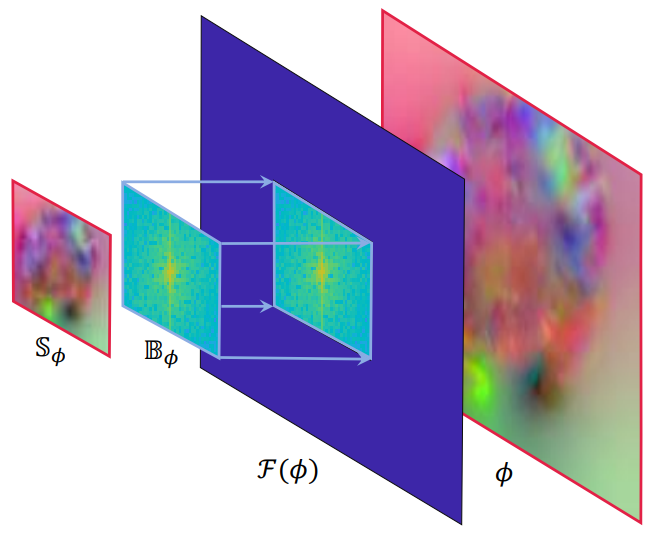
\includegraphics[width=.65\linewidth]{DecoderDisplacementField.png} 
	\caption{Reconstruction of the band-limited displacement field via the decoder taken from~\cite{Fourier-Net+}. The band-limited representation $\mathbb{B}_\phi$ is padded with zeros to the desired spatial resolution $\mathcal{F}(\phi)$ and then transformed to the full-resolution displacement $\phi$ using an iDFT.}
	\label{fig:DecoderDisplacementField}
\end{figure} 

\subsubsection{Diffeomorphic Transforms} \label{SubSubSec:DiffeomorphicTransforms}
Diffeomorphic deformations are differentiable and invertible, thus preserving topology, which is a desirable property for transformations. $\phi: \mathbb{R}^N \rightarrow \mathbb{R}^N$ represents the deformation that maps the coordinates from one image to coordinates in another image, as long as both images have the dimension $N$. When using a stationary velocity field representation like e.g. \emph{DARTEL}~\cite{DARTEL}, the deformation field is defined through the following ordinary differential equation (ODE)~\cite{Dalca2018}:
\begin{equation}
	\frac{\partial \phi^{(t)}}{\partial t} = v(\phi^{(t)}),
\end{equation}
where $\phi^{(0)} = \text{Id}$ is the identity transformation and $t$ is time. The final registration field $\phi^{(1)}$ can be obtained by integrating the stationary velocity field $v$ over $t = [0, 1]$. This is typically done by integration numerically using scaling and squaring~\cite{ScaleAndSquare}. The integration of a stationary ODE represents a one-parameter subgroup of diffeomorphisms. In group theory, $v$ is a member of the Lie algebra and is exponentiated to produce $\text{exp}(v) = \phi^{(1)}$, which is also a member of the Lie group. From the properties of one-parameter subgroups, for any scalars $t$ and $t'$, $\text{exp}((t + t') \cdot v) = \text{exp}(t \cdot v) \circ \text{exp}(t' \cdot v)$, where $\circ$ is a composition map associated with the Lie group. Starting from $\phi^{({1/2}^T)} = p + v(p)$ where $p$ is a map of spatial locations, we use the recurrence $\phi^{({1/2})^{t  1}} = \phi^{({1/2}^t)} \circ \phi^{({1/2}^t)}$ to obtain $\phi^1 = \phi^{(1/2)} \circ \phi^{(1/2)}$. $T$ is chosen so that $v \approx 0$~\cite{Dalca2018}. \\
As diffeomorphic deformations are defined as smooth and invertible deformations, the output of the iDFT layer in \emph{Fourier-Net} can be regarded as a stationary velocity field $v$ instead of a displacement field $\phi$. In Figure~\ref{fig:Fourier-Net} scaling and squaring layers are visualized. These apply the diffeomorphic transformation in three steps~\cite{ScaleAndSquare}:
\begin{enumerate}
	\item Scaling: Divide the velocity field $v$ by a factor $2^N$ , so that $\frac{v}{2^N}$ is close to zero (depending on the desired accuracy).
	\item Exponentiation: Compute $\text{exp}\big(\frac{v}{2^N}\big) = \phi^{(1)}\big(\frac{v}{2^N}\big)$ with a first-order explicit numerical scheme.
	\item Squaring: $N$ recursive squarings of $\phi^{(1)}\big(\frac{1}{2^N}\big) = \text{exp}\big(\frac{v}{2^N}\big)$ to yield an accurate estimation of $\phi^{(1)}(1) = \phi^{(1)}\big(\frac{1}{2^N}\big)^{2^N} = \text{exp}\big(\frac{v}{2^N}\big)^{2^N} = \text{exp}(v)$.
\end{enumerate}
Thus, the diffeomorphic deformation can be efficiently calculated. When used, the specific version is then called \emph{Fourier-Net Diff} to differentiate it from the baseline version.


\subsubsection{Spatial Transformer} \label{SubSubSec:SpatialTransformer}
The warping layer of \emph{Fourier-Net} utilizes the \emph{Spatial Transformer}~\cite{SpatialTransformer}, which allows for spatial image manipulation within the network. This is a differentiable and learnable module for neural networks which applies a spatial transformation to a feature map during a single forward pass. The spatial transformer mechanism is split into three parts as seen in Figure~\ref{fig:SpatialTransformer}. First is the localization network, which takes the input and outputs the parameters for the transformation. These are then used to create a sample grid using the grid generator. Lastly, the sampler produces the output feature map based on the input at the grid points.\\
From the input feature map $U \in \mathbb{R}^{H \times W \times C}$ with width $W$, height $H$ and channels $C$ the localization network $f_{\text{loc}}$ computes the parameters $\theta = f_{\text{loc}}(U)$ of the transformation $\mathcal{T}_\theta$ which is later applied to the feature map. Thus the size of $\theta$ varies depending on the transformation. 
%(e.g. 6D for an affine transformation). 
The localization network function can both be implemented as a fully-connected network or as a CNN, but should include a final regression layer to produce the transformation parameters.\\
In order to warp the input feature map, each output pixel is computed by applying a sampling kernel centered at a particular location in the input feature map. The output pixels are defined to lie on a regular grid $G = {G_i}$ of pixels, forming an output feature map $V \in \mathbb{R}^{H' \times W' \times C}$, where $H'$ and $W'$ are the height and width of the grid with C again being the number of channels, which is the same for input and output.\\
In order to perform a spatial transformation of the input feature map $U$, the sampler must take the set of sampling points $\mathcal{T}_\theta(G)$, along and produce the sampled output feature map $V$. Each coordinate $(x_i^s, y_i^s)$ in $\mathcal{T}_\theta(G)$ defines the spatial location in the input where a sampling kernel is applied to get the value at a particular pixel in the output:
\begin{equation}
	V_i^c = \sum^{H}_{n} \sum^{W}_{m} U_{nm}^c k(x_i^s - m; \Phi_x) k(y_i^s - n; \Phi_y),
\end{equation}
with $\Phi_x$ and $\Phi_y$ being the parameters for a generic sampling  kernel $k$ that defines the image interpolation, $U_{nm}^c$ is the value of the input feature maps at location $(n,m)$ in the channel $c \in [1, ..., C]$ and $V_i^c$ is the value for every pixel $i \in [1, ..., H'W']$ for the output feature map. Any sampling kernel can be used, as long as (sub-) gradients can be defined with respect to $(x_i^s, y_i^s)$ to allow the loss gradients to flow back not only to the input feature map, but also to the sampling grid coordinates and therefore back to the transformation parameters $\theta$ and localization network, thus enabling back-propagation~\cite{SpatialTransformer}.

\begin{figure}[h] %tpb
	\centering
	\graphicspath{{images/}{\main/images/}}
	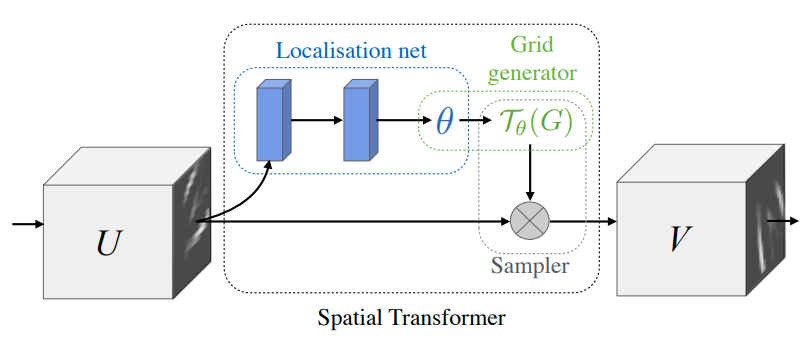
\includegraphics[width=\linewidth]{SpatialTransformer.png} 
	\caption{Architecture of the \emph{Spatial Transformer} taken from~\cite{SpatialTransformer}. The input feature map $U$ is passed to a localization network which outputs the transformation parameters $\theta$. The regular spatial grid $G$ over $V$ is transformed to the sampling grid $\mathcal{T}_\theta(G)$, which is applied to $U$ producing the warped output feature map $V$.}
	\label{fig:SpatialTransformer}
\end{figure}


\subsubsection{Loss Function} \label{SubSubSec:LossFunction}
The loss function consists of two parts to enable unsupervised learning, which are balanced using the scalar parameter $\lambda$. The first, $\mathcal{L}_{1}$, measures the similarity between the fixed image and the moving image after warping, while the second, $\mathcal{L}_{2}$, ensures a smooth displacement field. Thus, the unsupervised loss $\mathcal{L}$ can be calculated as follows:
\begin{equation}	\label{eq:unsupervisedLoss}
	\begin{split} 
		\mathcal{L}(\Theta) &= \min  \bigg( \mathcal{L}_{1} (\phi(\Theta))  + \lambda \cdot \mathcal{L}_{2} (\phi(\Theta)) \bigg) \\
		&= \min  \bigg( \mathcal{L}_{1} (v(\Theta))  + \lambda \cdot \mathcal{L}_{2} (v(\Theta)) \bigg),
	\end{split}
\end{equation}
for both displacement fields $\phi$ and velocity fields $v$. The first part of the loss function consists of:
\begin{equation} \label{eq:L1-LossDisp}
	\mathcal{L}_{1} (\phi(\Theta)) = \frac{1}{N} \sum^{N}_{i=1} \mathcal{L}_{Sim} (M_i \circ (\phi_i(\Theta) + \text{Id}) - F_i),
\end{equation}
where $\circ$ denotes the warping operation, $N$ the number of training pairs with moving images $M_i$ and fixed images $F_i$, $\Theta$ the network parameters, $\phi_i$ the displacement field, Id the identity grid. $\mathcal{L}_{Sim}$ determines the similarity between warped moving images and fixed images via MSE or NCC, and the second term of the unsupervised loss, $\mathcal{L}_{2}$, defines the smoothness regularization function that controls smoothness of the displacement fields:
\begin{equation} \label{eq:L2-LossDisp}
	\mathcal{L}_{2} (\phi(\Theta)) = \frac{1}{N} \sum^{N}_{i=1} || \nabla \phi_i(\Theta) ||^2_2,
\end{equation}
with $\nabla$ denoting the first order gradient and $|| \cdot ||_2^2$ denoting the squared $L_2$-Norm. \\
When using the squaring and scaling layers, thus making the deformation of the moving image diffeomorphic, the loss needs to be modified by replacing the displacement field $\theta$ with the velocity field $v$. Thus, both parts of the of the loss function need to be changed:
\begin{equation}	\label{eq:L1-LossVeloc}
	\mathcal{L}_{1} (v(\Theta)) = \frac{1}{N} \sum^{N}_{i=1} \mathcal{L}_{Sim} (M_i \circ Exp(v_i(\Theta) - F_i),
\end{equation}
\begin{equation} \label{eq:L2-LossVeloc}
	\mathcal{L}_{2} (v(\Theta)) = \frac{1}{N} \sum^{N}_{i=1} || \nabla v_i(\Theta) ||^2_2  \bigg .
\end{equation}


\subsection{Fourier Net+} \label{SubSec:Fourier-Net+}
\emph{Fourier-Net+}, as the name suggests, is an extension of Fourier-Net which takes the band-limited spatial representation of the images as input, instead of their original full-resolution counterparts. This leads to further reduction in the number of convolutional layers in the contracting path of the network, resulting in a decrease of parameters, memory usage, and computational operations. This makes \emph{Fourier-Net+} even more efficient than its predecessor~\cite{Fourier-Net+}.\\
As seen in Figure~\ref{fig:Fourier-Net+}, the network architecture is almost the same as for \emph{Fourier-Net} (see Figure~\ref{fig:Fourier-Net} for comparison). However, while the decoder, and thus the loss function, remain the same, the encoder is slightly altered to make the network even more efficient. For this, similarly to the decoder, a DFT is used, however this time the idea is applied to the input images. These are first transformed into the Fourier domain, then low-pass filtered by center-cropping and finally reconstructed from their band-limited representation back into the spatial domain via an iDFT. The two images, now compressed, are the input for the encoder of \emph{Fourier-Net}, meaning the CNN and following DFT. However, due to the band-limiting before the CNN, the latter can be made much more light-weight, thus reducing computational cost. This is visualized in Figure~\ref{fig:Fourier-Net+CNN}. Thus, \emph{Fourier-Net+} too is overall lighter than the baseline \emph{Fourier-Net} in terms of the number of parameters and computations. However, such a light network may face limitations in accurately capturing complex deformations. To counter this potential weakness, the authors propose a cascaded version of \emph{Fourier-Net+}, which uses multiple versions of \emph{Fourier-Net+} cascaded one after the other to achieve a better overall displacement field~\cite{Fourier-Net+}. A schematic for this can be seen in Figure~\ref{fig:Fourier-Net+Cascaded}.

\begin{figure}[h] %tpb
	\centering
	\graphicspath{{images/}{\main/images/}}
	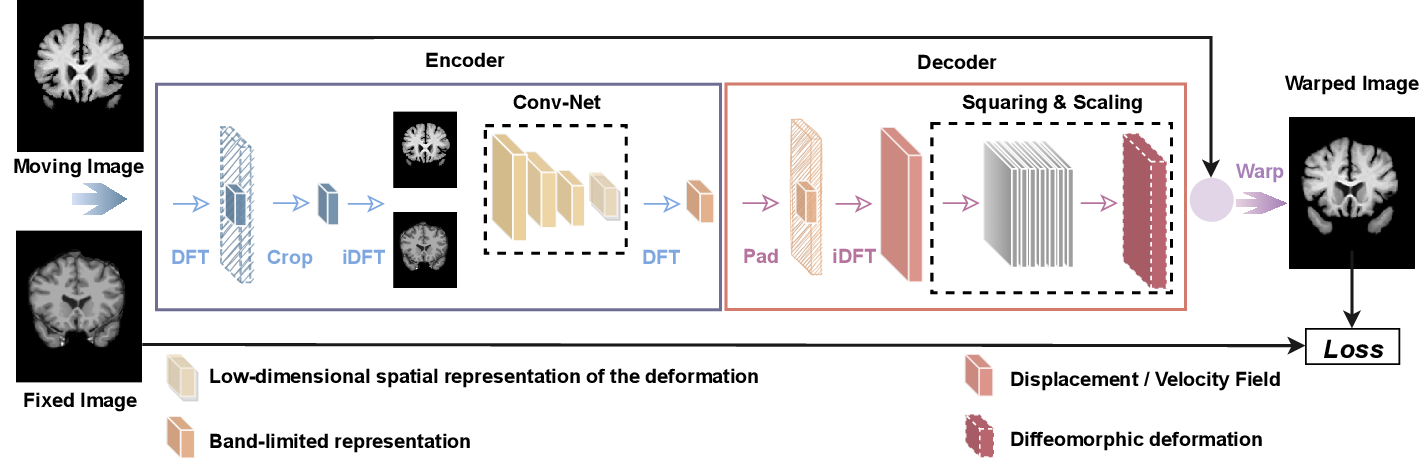
\includegraphics[width=\linewidth]{ArchitectureFourier-Net+.png} 
	\caption{Architecture of \emph{Fourier-Net+} taken from~\cite{Fourier-Net+}. The encoder has a additional compression step to reduce the input size of the images compared to \emph{Fourier-Net}. This is achieved by center-cropping the k-space of the images obtained via a DFT and then reconstructing them via an iDFT to get a compressed version of the inputs without the higher frequencies present. The rest of the network is the same as for \emph{Fourier-Net}.}
	\label{fig:Fourier-Net+}
\end{figure}

\subsubsection{Changes to the Encoder} \label{SubSubSec:ChangesEncoder}
In order to further reduce the amount of computational operations, \emph{Fourier-Net+} discards the early layers of the encoder. Instead, a DFT $\mathcal{F}(I_M)$ followed by a center-crop to produce the band-limited representation $\mathbb{B}_{I_M}$ in the frequency domain and iDFT are used to get the spatial patch $\mathbb{S}_{I_M}$, while the rest of the encoder from \emph{Fourier-Net} stays the same. The input $I_M$ is thus compressed to a lower resolution (i.e. band-limited) using the frequency space, which reduces the computational cost. This process is visualized in Figure~\ref{fig:Fourier-Net+EncoderCompression}. The encoder of \emph{Fourier-Net+} has several convolutional layers less in the contracting path compared to \emph{Fourier-Net}, which leads to a further accelerated registration process while reducing the memory footprint. These advantages are visualized in Figure~\ref{fig:Fourier-Net+CNN} where the amount of different layers between a conventional U-Net, \emph{Fourier-Net} (with the smaller decoder) and \emph{Fourier-Net+} (with a smaller encoder and decoder) are shown.

\begin{figure}[h] %tpb
	\centering
	\graphicspath{{images/}{\main/images/}}
	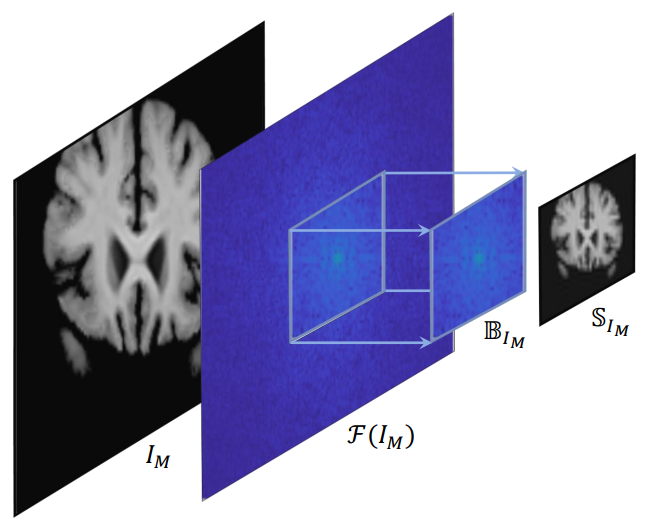
\includegraphics[width=.65\linewidth]{CompressionEncoder.png} 
	\caption{Compression in the frequency domain of the encoder used in \emph{Fourier-Net+} taken from~\cite{Fourier-Net+}. The frequencies $\mathcal{F}(I_M)$ are obtained via a DFT and then center-cropped to obtain a band-limited version $\mathbb{B}_{I_M}$. The compressed image $\mathbb{S}_{I_M}$ is then reconstructed via a iDFT.}
	\label{fig:Fourier-Net+EncoderCompression}
\end{figure}

\begin{figure}[h] %tpb
	\centering
	\graphicspath{{images/}{\main/images/}}
	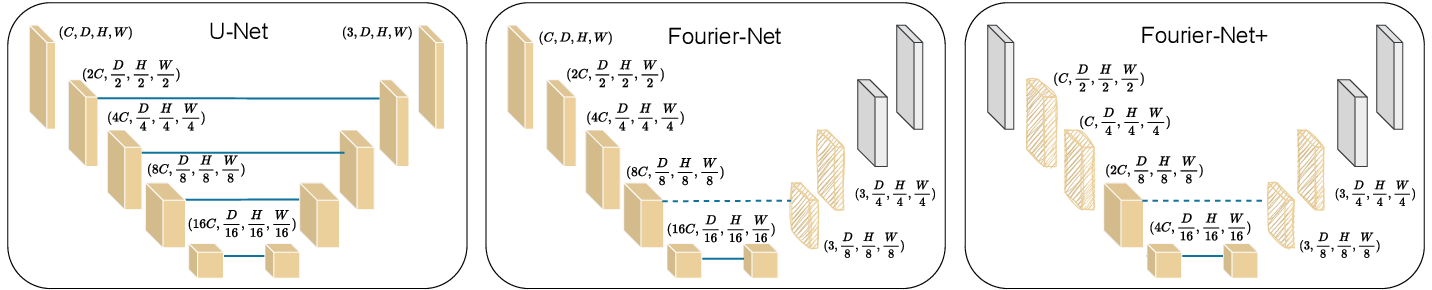
\includegraphics[width=\linewidth]{ArchitectureFourier-Net+CNN.png} 
	\caption{Architecture of the CNN for a typical U-Net, \emph{Fourier-Net} and \emph{Fourier-Net+} taken from~\cite{Fourier-Net+}. The latter have far less trainable network parameters due to only computing a band-limited displacement. \emph{Fourier-Net+} additionally has a smaller encoder due to compressing the input images.} % making it even more efficient
	\label{fig:Fourier-Net+CNN}
\end{figure}

\subsubsection{Effects of Cascading} \label{SubSubSec:EffectsCascading}
As seen in the previous section, \emph{Fourier-Net+} is lighter than \emph{Fourier-Net} due to the band-limited representation of both images and deformations lowering the number of parameters and computations. This, however, can lead to limitations when trying to accurately capture complex deformations. To this end, a cascaded version of \emph{Fourier-Net+} called \emph{K$\times$Fourier-Net+} (see Figure~\ref{fig:Fourier-Net+Cascaded}), with $K$ denoting the amount of cascades, can be used where the the warped image of one cascade is used as the moving image of the next. It is important to note that the weights are not shared between cascades. The squaring and scaling layers, in case a diffeomorphic deformation is wanted, are applied after the last cascade. The same is true for the calculation of the loss function.\\
In order to more accurately describe this version of \emph{Fourier-Net+} one can look at the in- and outputs of the different cascades. The first cascade of \emph{K$\times$Fourier-Net+} has the moving image $I_M$ and fixed image $I_F$ as inputs. While the latter always stays the same for all cascades the warped image $I_M^{w(1)}$ from the first cascade is used as input for the second cascade instead of the original moving image. Thus, in general $I_M^{w(k-1)}$ and $I_F$ are the inputs for a cascade $k \in [1, K]$ with output $\delta \phi^{(k)}$. Furthermore, $I_M^{w(k)}$ can be defined as:
\begin{equation}
	I_M^{w(k)} = ((((I_M \circ \delta \phi^{(1)}) \circ \delta \phi^{(2)}) \circ \dots ) \circ \delta \phi^{(k-1)}) \circ \delta \phi^{(k)} = I_M \circ  \phi^{(k)},
\end{equation}
with $\phi^{(k)}$ being the displacement field computed by composing the outputs of the first cascade up to the $k$-th cascade:
\begin{equation}
	\phi^{(k)} = \delta \phi^{(1)} \circ \delta \phi^{(2)} \circ \dots \circ \delta \phi^{(k-1)} \circ \delta \phi^{(k)}.
\end{equation}
Thus, the output displacement field of the $K$-th cascade $\phi^{(K)}$ is the final displacement which is then used to warp $I_M$, the original moving image, in order to compute the loss~\cite{Fourier-Net+}.

\begin{figure}[h] %tpb
	\centering
	\graphicspath{{images/}{\main/images/}}
	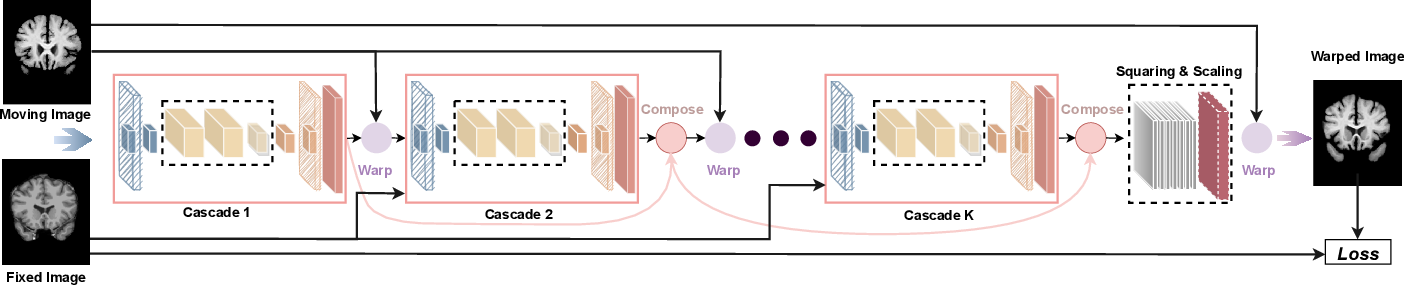
\includegraphics[width=\linewidth]{ArchitectureFourier-Net+Cascaded.png} 
	\caption{Cascaded version of \emph{Fourier-Net+} taken from~\cite{Fourier-Net+}. Multiple instances of \emph{Fourier-Net+} can be cascaded with independent weights for better performance as the network itself is very memory efficient.}
	\label{fig:Fourier-Net+Cascaded}
\end{figure}


\section{Datasets}	\label{Sec:Datasets}
In the following chapter, the datasets used in this thesis are presented. The \emph{Automated Cardiac Diagnosis Challenge (ACDC)} dataset~\cite{ACDC} from the \emph{MICCAI 2017} conference was mainly used for ablation studies and parameter tests. While it contains no k-space data, segmentations are given for the end-systolic and end-diastolic frames of the test set, which can be used to evaluate the registration performance using the Dice score. \\
The \emph{CMRxRecon} dataset~\cite{CMRxRecon} from the \emph{CMRxRecon2023} challenge specializes in CMR imaging. It was used for downstream-tests regarding MR image reconstruction. The cardiac MRI k-space data was used for the evaluation motion-compensated reconstruction pipeline. It contains subsampled data, but does not provide segmentations for multi-coil data.

\subsection{ACDC Dataset} \label{SubSec:ACDC}
The \emph{ACDC} dataset contains cardiac cine MRI short-axis data from 150 subjects that were divided into 5 subgroups (4 pathological, 1 healthy). For each subject systolic (see Figure~\ref{fig:Image_ACDC_systolic}) and diastolic frames (see Figure~\ref{fig:Image_ACDC_diastolic}) are provided with corresponding segmentations (see Figure~\ref{fig:Segmentation_ACDC_systolic} and ~\ref{fig:Segmentation_ACDC_diastolic}), which enables direct comparison via e.g. the Dice score. The segmentations contain only four values with 0, 1, 2 and 3 representing pixels located in the background, in the right ventricle (RV) cavity, in the myocardium, and in the left ventricle (LV) cavity. The frames themselves are 3D volumes with size $216 \times 256 \times 10$, thus ten image slices can be extracted which each have size $216 \times 256$. The same holds true for the segmentation, which means that both the image data and segmentations can generated in the same manner.\\
For the training data, the original 4D data was used as we do not require the segmentations for the end-systolic and end-diastolic frames. As the 4D data has size $216 \times 256 \times 10 \times 30$ we can extract 30 frames for each of the ten slices. These can be sorted into 251376 image pairs for training. For the validation and test data the end-systolic and end-diastolic frames with their segmentations were used giving us 641 image pairs each.\\
As the dataset only contained images reconstructed from fully sampled data, the data had to manually be subsampled. This was done by first obtaining the k-space data via a FFT and then subsampling the k-space for $=4$, $R=8$ and $R=10$ before going back to image space using a iFFT. This naive reconstruction lead to the typical artifacts (see Figure~\ref{fig:ManuelSubsampling_ACDC}) that the networks will be tested against.

\begin{figure}[h]%tpb
	\centering
	\begin{subfigure}{0.45\textwidth}
    		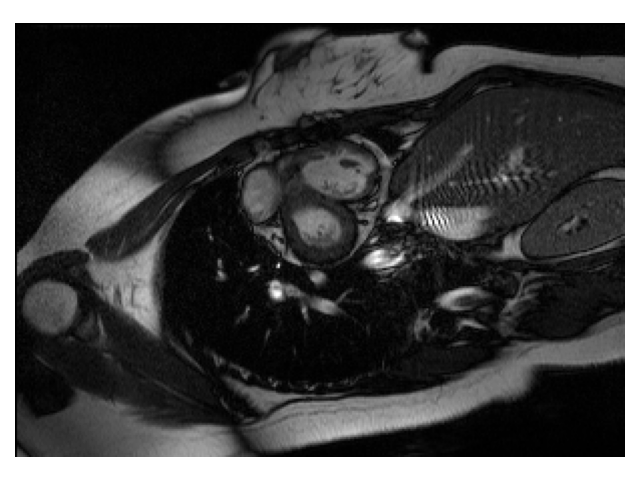
\includegraphics[width=\textwidth]{./Images/Image_ACDC_systolic.png}
    		\caption{Image of systolic phase.}
    		\label{fig:Image_ACDC_systolic}
	\end{subfigure}
	\hfill
	\begin{subfigure}{0.45\textwidth}
    		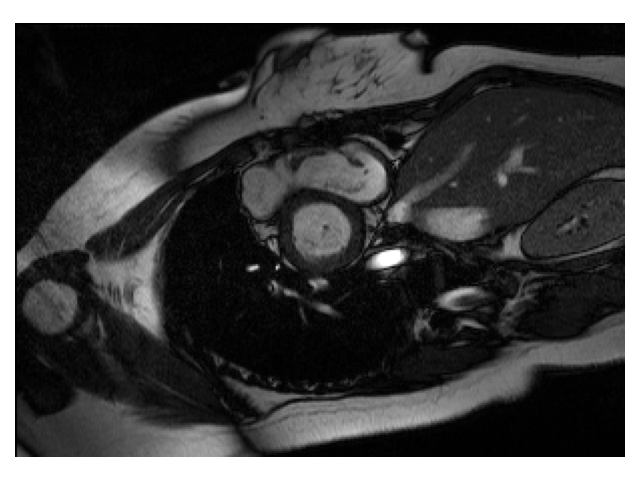
\includegraphics[width=\textwidth]{./Images/Image_ACDC_diastolic.png}
    		\caption{Image of diastolic phase.}
    		\label{fig:Image_ACDC_diastolic}
	\end{subfigure} 
	\\
	\begin{subfigure}{0.45\textwidth}
    		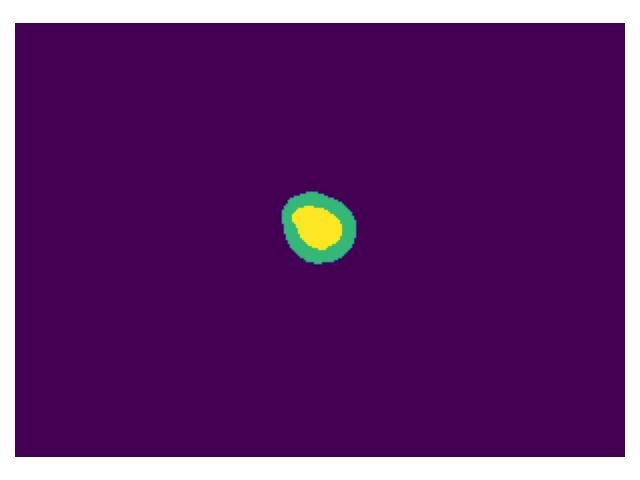
\includegraphics[width=\textwidth]{./Images/Segmentation_ACDC_systolic.png}
    		\caption{Segmentation of systolic phase.}
    		\label{fig:Segmentation_ACDC_systolic}
	\end{subfigure}
	\hfill
	\begin{subfigure}{0.45\textwidth}
    		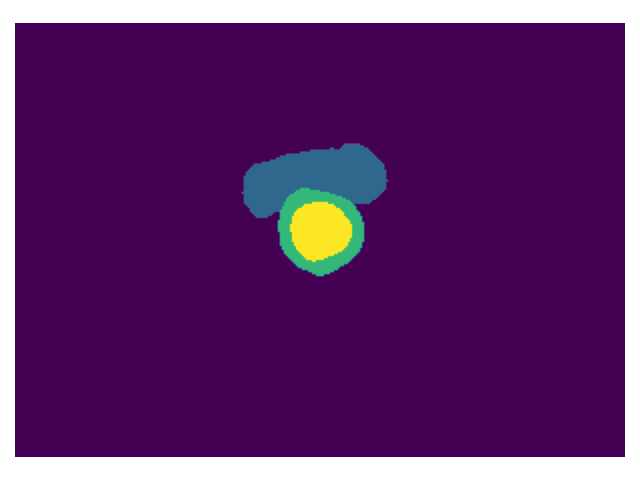
\includegraphics[width=\textwidth]{./Images/Segmentation_ACDC_diastolic.png}
    		\caption{Segmentation of diastolic phase.}
    		\label{fig:Segmentation_ACDC_diastolic}
	\end{subfigure}
	\caption{Example images for systolic (a) and diastolic frames (b) with corresponding segmentations (c),(d) taken from the \emph{ACDC} dataset~\cite{ACDC}.}
	\label{fig:}
\end{figure}

\begin{figure}[h] %tpb
	\centering
	\begin{subfigure}{0.3\textwidth}
    		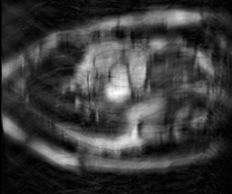
\includegraphics[width=\textwidth]{./Images/ManuelSubsampling_ACDC_R=4.png}
    		\caption{Manuel subsampling for $R=4$.}
    		\label{fig:ManuelSubsampling_ACDC_R=4}
	\end{subfigure}
	\hfill 
	\begin{subfigure}{0.3\textwidth}
    		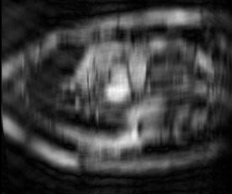
\includegraphics[width=\textwidth]{./Images/ManuelSubsampling_ACDC_R=8.png}
    		\caption{Manuel subsampling for $R=8$.}
    		\label{fig:ManuelSubsampling_ACDC_R=8}
	\end{subfigure}
	\hfill 
	\begin{subfigure}{0.3\textwidth}
    		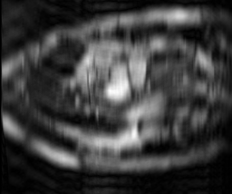
\includegraphics[width=\textwidth]{./Images/ManuelSubsampling_ACDC_R=10.png}
    		\caption{Manuel subsampling for $R=10$.}
    		\label{fig:ManuelSubsampling_ACDC_R=10}
	\end{subfigure}
	\caption{Example images for the manual subsampling $R=4$, $R=8$, and $R=10$ of the \emph{ACDC} data.}
	\label{fig:ManuelSubsampling_ACDC}
\end{figure}


\subsection{CMRxRecon Dataset} \label{SubSec:CMRxRecon}
The \emph{CMRxRecon} dataset includes 
%multi-contrast k-space data, consisting of cardiac cine, $\text{T}_1$/$\text{T}_2$-mapping, tagging, phase-contrast (i.e., flow2d), and dark-blood imaging
fully sampled and subsampled multi-coil k-space data, as well as auto-calibration lines from the center region. This includes imaging of different anatomical views like long-axis (2-chamber, 3-chamber, and 4-chamber) and short-axis (SAX). There is a total of 120 training data, 60 validation data, and 120 test data from healthy volunteers. In contrast to the \emph{ACDC} dataset, \emph{CMRxRecon} contains only the raw k-space data. One of the goals of the challenge is the reconstruction from subsampled k-space data, e.g. accelerated MRI scans.\\
As the data was recorded in the k-space (see Figure~\ref{fig:k-space}) and stored as \emph{.mat} files it first needs to reconstructed to images in order to use them for training and testing of neural networks. First, an iFFT needs to be performed to get from k-space to image space, however the multi-coil data needs further treatment. The effect of different coil sensitivities in their respective images can be seen in Figure~\ref{fig:Coils}, where each coil focuses on a specific area of the image. These images are then stitched together during reconstruction to produce a coil-combined image with great overall contrast. Often the simple RSS method is used where the resulting image is simply the root of the sum of the squared coil images~\cite{Roemer1990}. \\
%, while Figure~\ref{fig:ImageSlice} contains the complete reconstructed image. 
The dataset, as mentioned before, contains fully sampled as well as subsampled k-space data (see Figure~\ref{fig:fullySampled} and Figure~\ref{fig:subSampled}), with the latter being typically used to accelerate the MRI acquisition process. This is done by not using all of the available k-space data, but rather masking the signal to achieve the subsampling. The center region of the k-space is usually fully sampled, but the outer regions are subsampled depending on the sampling strategy~\cite{SamplingStrategies}. The dataset contains subsampled k-space data for 4x, 8x and 10x acceleration with the latter of course leading to more distortions in the reconstructed image as the subsampling can induce image reconstruction artifacts. This can be seen in Figure~\ref{fig:subSampledImage}, where the image reconstructed from 4x accelerated ($R=4$) k-space data seems blurred when compared to the fully sampled ($R=0$) one in Figure~\ref{fig:fullySampledImage}. \\
%An example image can be seen in Figure~\ref{fig:Subsampling} where the k-space of the original image is subsampled with a random mask leading to heavy blurring artifacts after the reconstruction.
For all experiments, the short-axis view data was used. As image sizes between patients can vary slightly, interpolation was used to standardize the images to a size of $246 \times 512$ to avoid further problems with e.g. 
%ensure coherent sizes between images to avoid problems with the network and 
loss calculation. Additionally, min-max-normalization is used to standardize the data range for all images to $[0,1]$. The reconstructed images were stored for every image slice for every patient. Thus, all frames for a specific image slice were in a single folder to enable easy access for later data load-in for frame-to-frame registration.

\begin{figure}[h]%tpb
	\centering
	\graphicspath{{images/}{\main/images/}}
	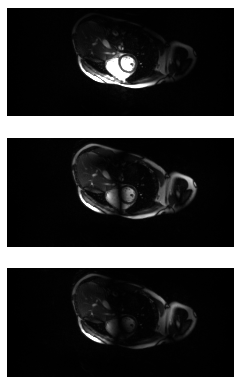
\includegraphics[width=\linewidth]{Coils.png} 
	\caption{MRI images for three different coils from the \emph{CMRxRecon} dataset~\cite{CMRxRecon}. The different sensitive areas can clearly be seen as they have significantly higher pixel values compared to the rest of the image. The background was cropped out from the images as the effect is not visible there. Note that the sensitivities are slightly corrupted as the coils were compressed to 10 coils for all the scans.}
	\label{fig:Coils}
\end{figure}


\begin{figure}[h]%tpb
	\centering
	\graphicspath{{images/}{\main/images/}}
	\begin{subfigure}{0.45\textwidth}
    		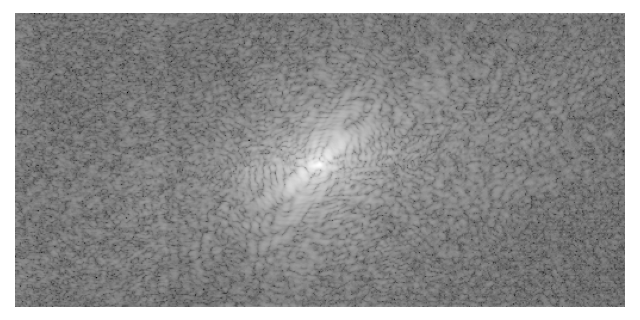
\includegraphics[width=\textwidth]{k-space_fullysampled.png}
    		\caption{A fully sampled k-space with low frequencies in the center and higher frequencies in the outer regions.}
    		\label{fig:fullySampled}
	\end{subfigure}
	\hfill
	\begin{subfigure}{0.45\textwidth}
    		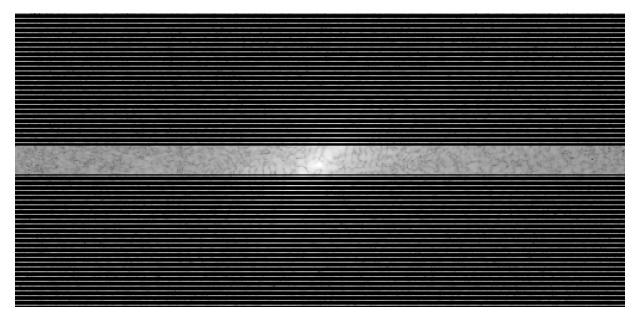
\includegraphics[width=\textwidth]{k-space_subsampled.png}
    		\caption{A 4x accelerated k-space. The center region remains fully sampled while higher frequencies are omitted.}
    		\label{fig:subSampled}
	\end{subfigure}\\
	\begin{subfigure}{0.45\textwidth}
    		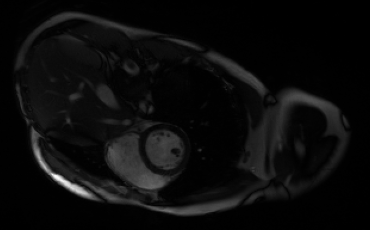
\includegraphics[width=\textwidth]{image_fullysampled.png}
    		\caption{Corresponding high quality image reconstructed from the fully sampled k-space.}
    		\label{fig:fullySampledImage}
	\end{subfigure}
	\hfill
	\begin{subfigure}{0.45\textwidth}
    		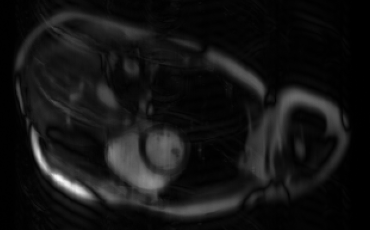
\includegraphics[width=\textwidth]{image_subsampled.png}
    		\caption{Corresponding image reconstructed from the subsampled k-space with blurring and aliasing artifacts.}
    		\label{fig:subSampledImage}
	\end{subfigure}
	\caption{Fully sampled and subsampled k-space data from the from the \emph{CMRxRecon} dataset~\cite{CMRxRecon} with corresponding images (empty background was cropped out).}
	\label{fig:k-space}
\end{figure}

\subsection{Simulated Motion} \label{SubSec:SimulatedMotion}
In order to test the motion-compensated reconstruction pipeline, strongly motion-corrupted data is needed. As none of the datasets described previously meet these demands, the motion needed to be simulated manually. To simulate this motion or mis-triggering, two different strategies were used. First, line swapping in the k-space, and second, non-linear lung transformations.

\subsubsection{K-space Line Swapping}
First, a strategy similar to~\cite{Oksuz2020} was used, swapping $z$ k-space lines between the frames in k-space. The frames used for this all stem from the same slice and the information is swapped for all coils. The new fully sampled frames were then subsampled to the needed acceleration using the subsampling masks. Then, an iFT and RSS was used to generate the corrupted images. An example for $z=\{16,32\}$ can be seen in Figure~\ref{fig:LineSwapping}. 


% Line Swapping next to each other
\begin{figure}[h] %tpb
	\centering
	\begin{subfigure}{0.325\textwidth}
    		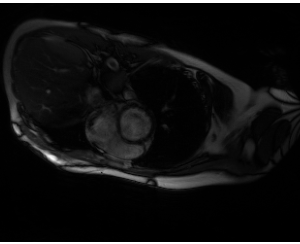
\includegraphics[width=\textwidth]{./Images/LineSwappingOriginal.png}
    		\caption{Original image.}
    		\label{fig:LineSwappingOriginal}
	\end{subfigure}
	\hfill
	\begin{subfigure}{0.325\textwidth}
    		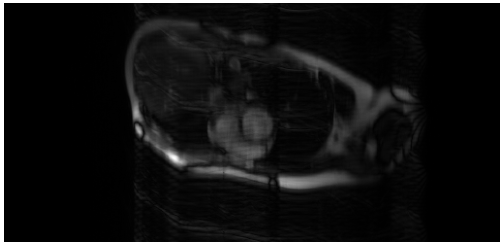
\includegraphics[width=\textwidth]{./Images/LineSwapping16.png}
    		\caption{Line swapping $z=16$.}
    		\label{fig:LineSwapping16}
	\end{subfigure}
	\hfill
	\begin{subfigure}{0.325\textwidth}
    		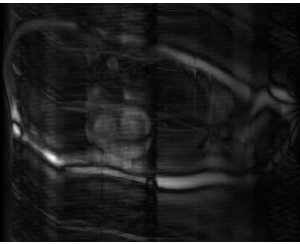
\includegraphics[width=\textwidth]{./Images/LineSwapping32.png}
    		\caption{Line swapping $z=32$.}
    		\label{fig:LineSwapping32}
	\end{subfigure}
	\caption{Examples for line swapping for $z=\{16,32\}$ with $R=4$ subsampling compared to the original fully sampled image.}
	\label{fig:LineSwapping}
\end{figure}

%% Line Swapping under each other
%\begin{figure}[h] %tpb
%	\centering
%	\begin{subfigure}{0.8\textwidth}
%    		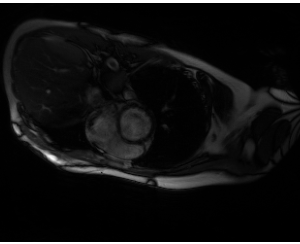
\includegraphics[width=\textwidth]{./Images/LineSwappingOriginal.png}
%    		\caption{Original image.}
%    		\label{fig:LineSwappingOriginal}
%	\end{subfigure}
%	\\
%	\begin{subfigure}{0.8\textwidth}
%    		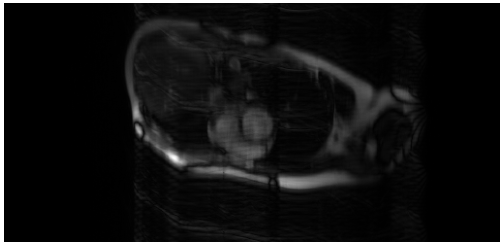
\includegraphics[width=\textwidth]{./Images/LineSwapping16.png}
%    		\caption{Line swapping $z=16$.}
%    		\label{fig:LineSwapping16}
%	\end{subfigure}
%	\\
%	\begin{subfigure}{0.8\textwidth}
%    		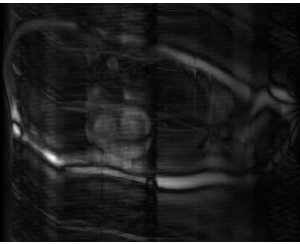
\includegraphics[width=\textwidth]{./Images/LineSwapping32.png}
%    		\caption{Line swapping $z=32$.}
%    		\label{fig:LineSwapping32}
%	\end{subfigure}
%	\caption{Examples for line swapping with $R=4$ subsampling compared to the original fully sampled image.}
%	\label{fig:LineSwapping}
%\end{figure}

\subsubsection{Non-Linear Lung Transformations}
Second, a simulation of non-linear lung movement was performed by randomly deforming the images and then generating the motion-corrupted k-space data from them. For this, a random displacement generator from~\cite{LAPNet} was used to generate random displacements in image space with a maximum velocity of 0.1. These displacements were then applied to each coil image before using an FT to convert from image to k-space, thereby modeling lung motion by expanding a cardiac time point into different respiratory time points for the multi-coil k-space data. This was done for $L=4$ additional lung motion frames for each cardiac frame. An example of such additional frames with artificial lung movement can be as seen in Figure~\ref{fig:LungMotion}.

% lung motion 2x2
\begin{figure}[h] %tpb 
	\centering
	\begin{subfigure}{0.475\textwidth}
    		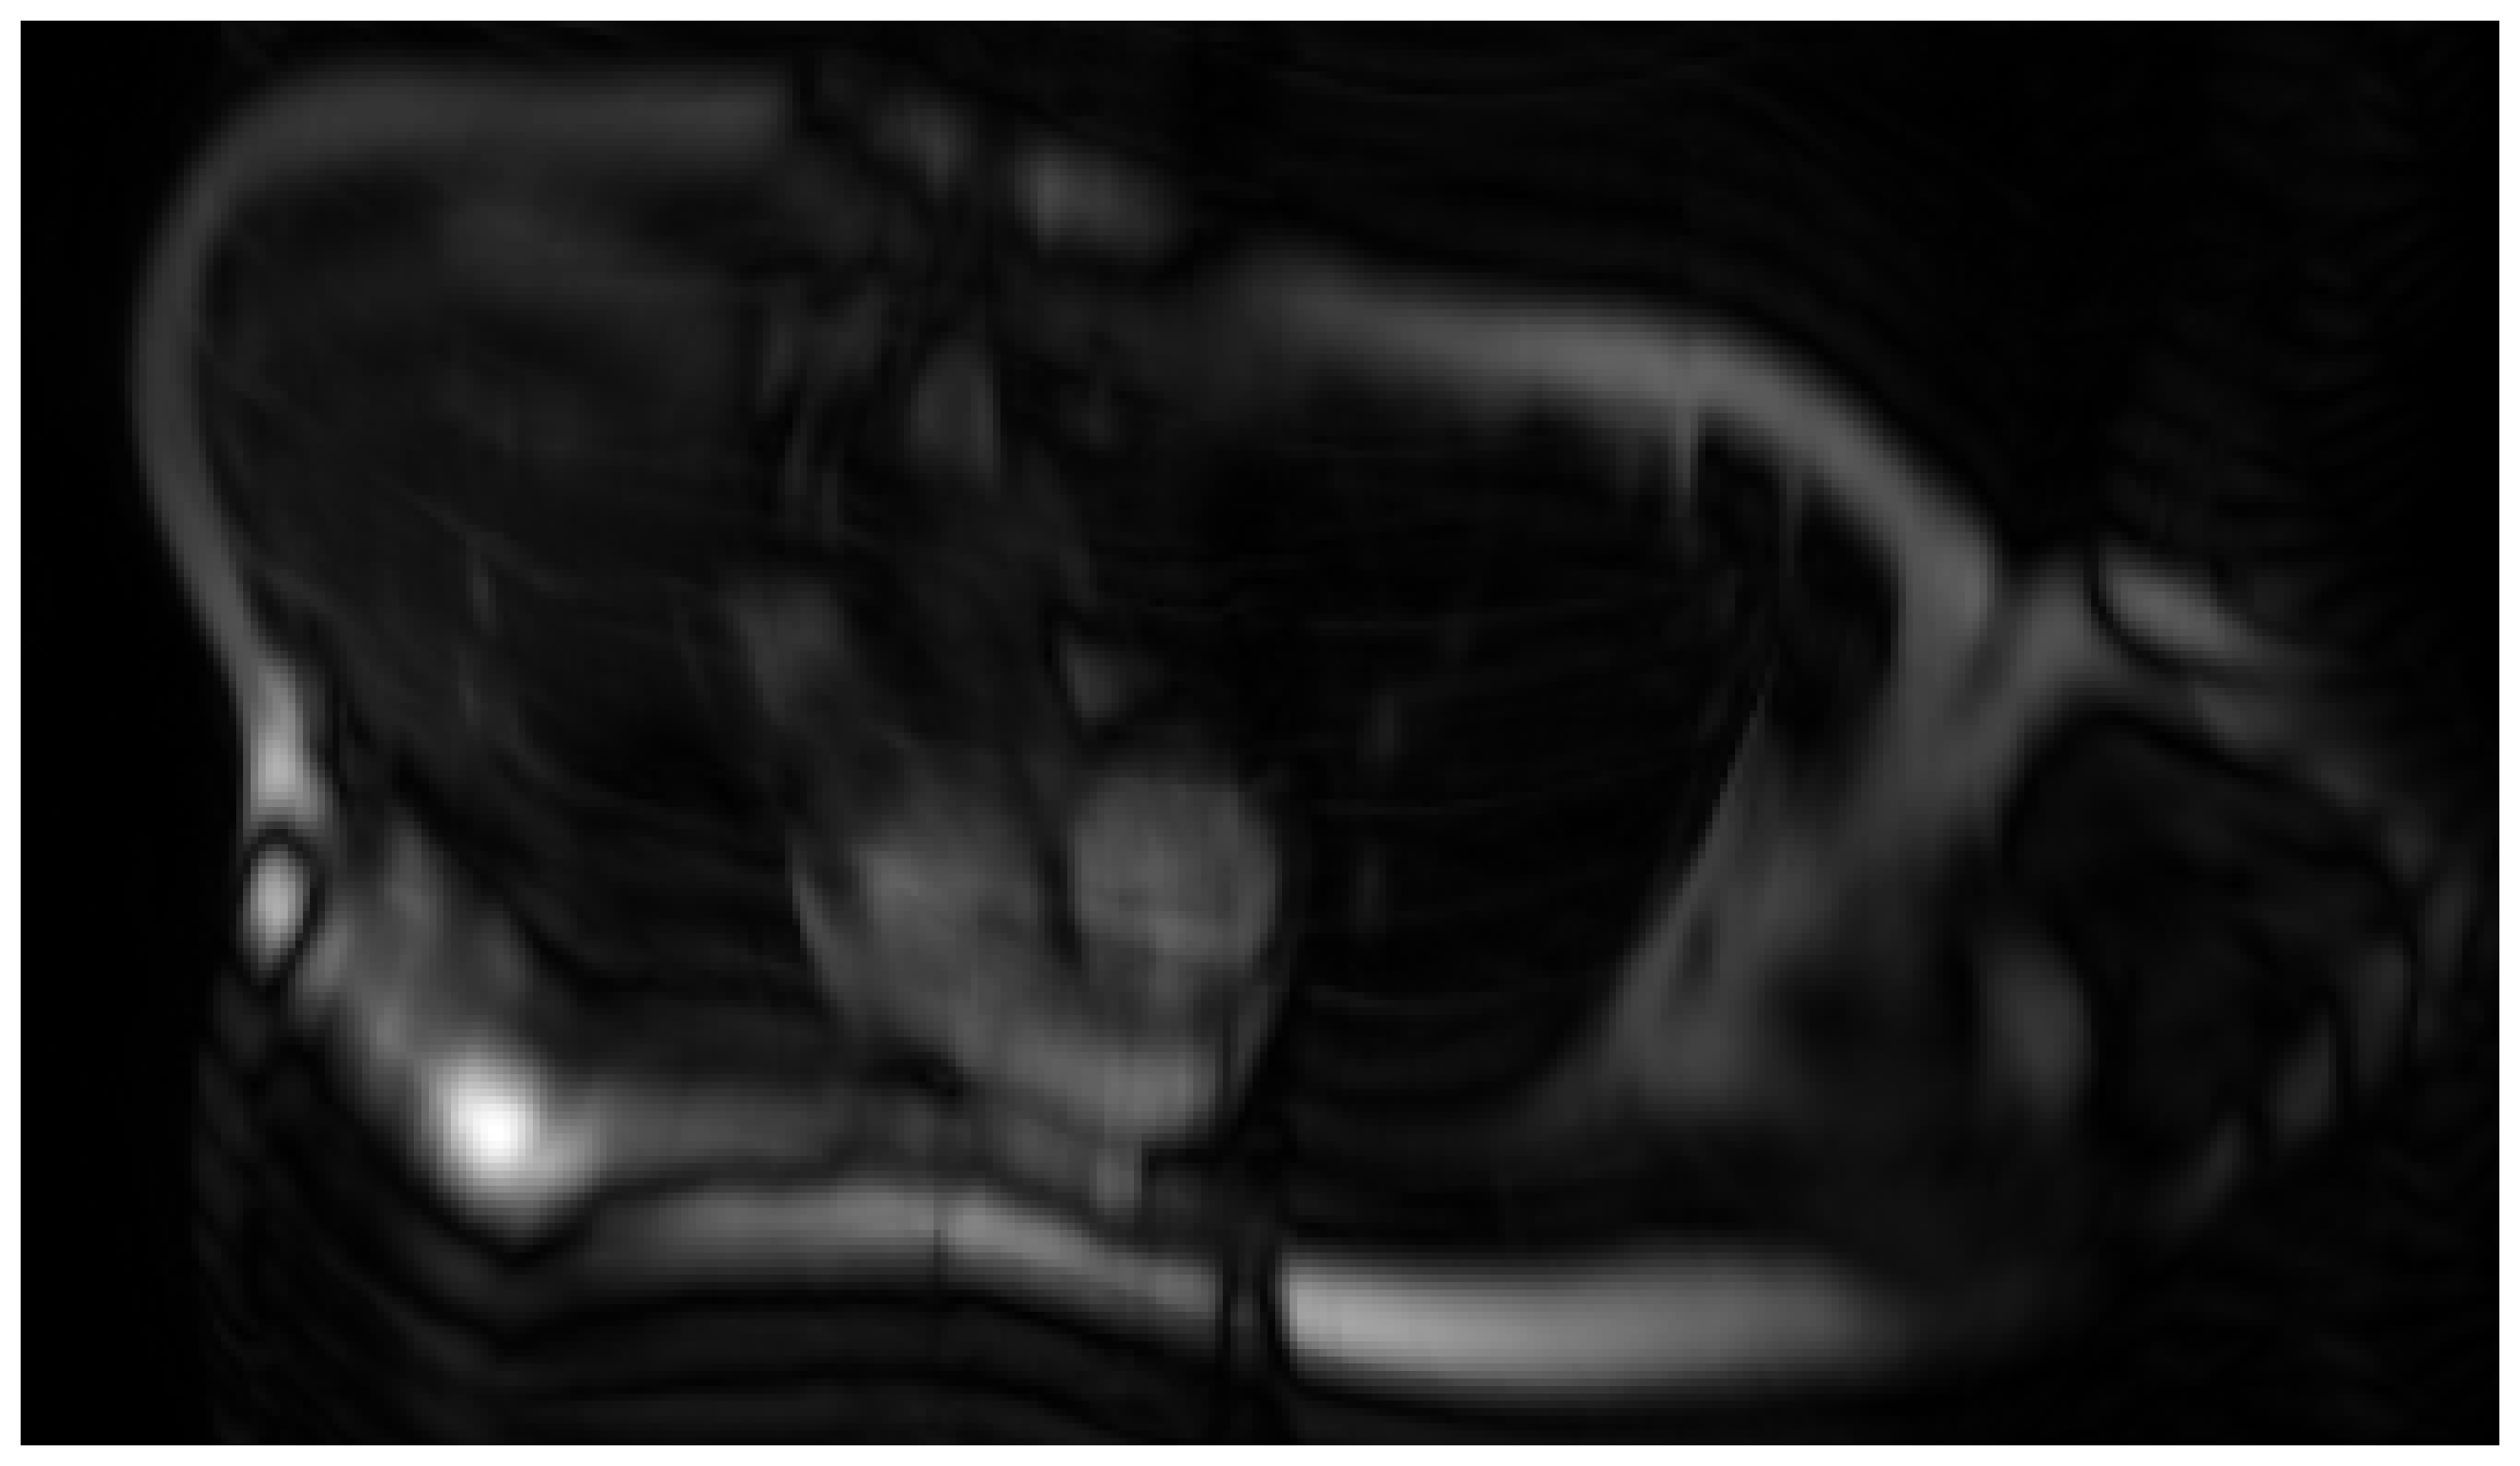
\includegraphics[width=\textwidth]{./Images/LungMotion1.png}
    		%\caption{First subfigure.}
    		\label{fig:LungMotion1}
	\end{subfigure}
	\hfill
	\begin{subfigure}{0.475\textwidth}
    		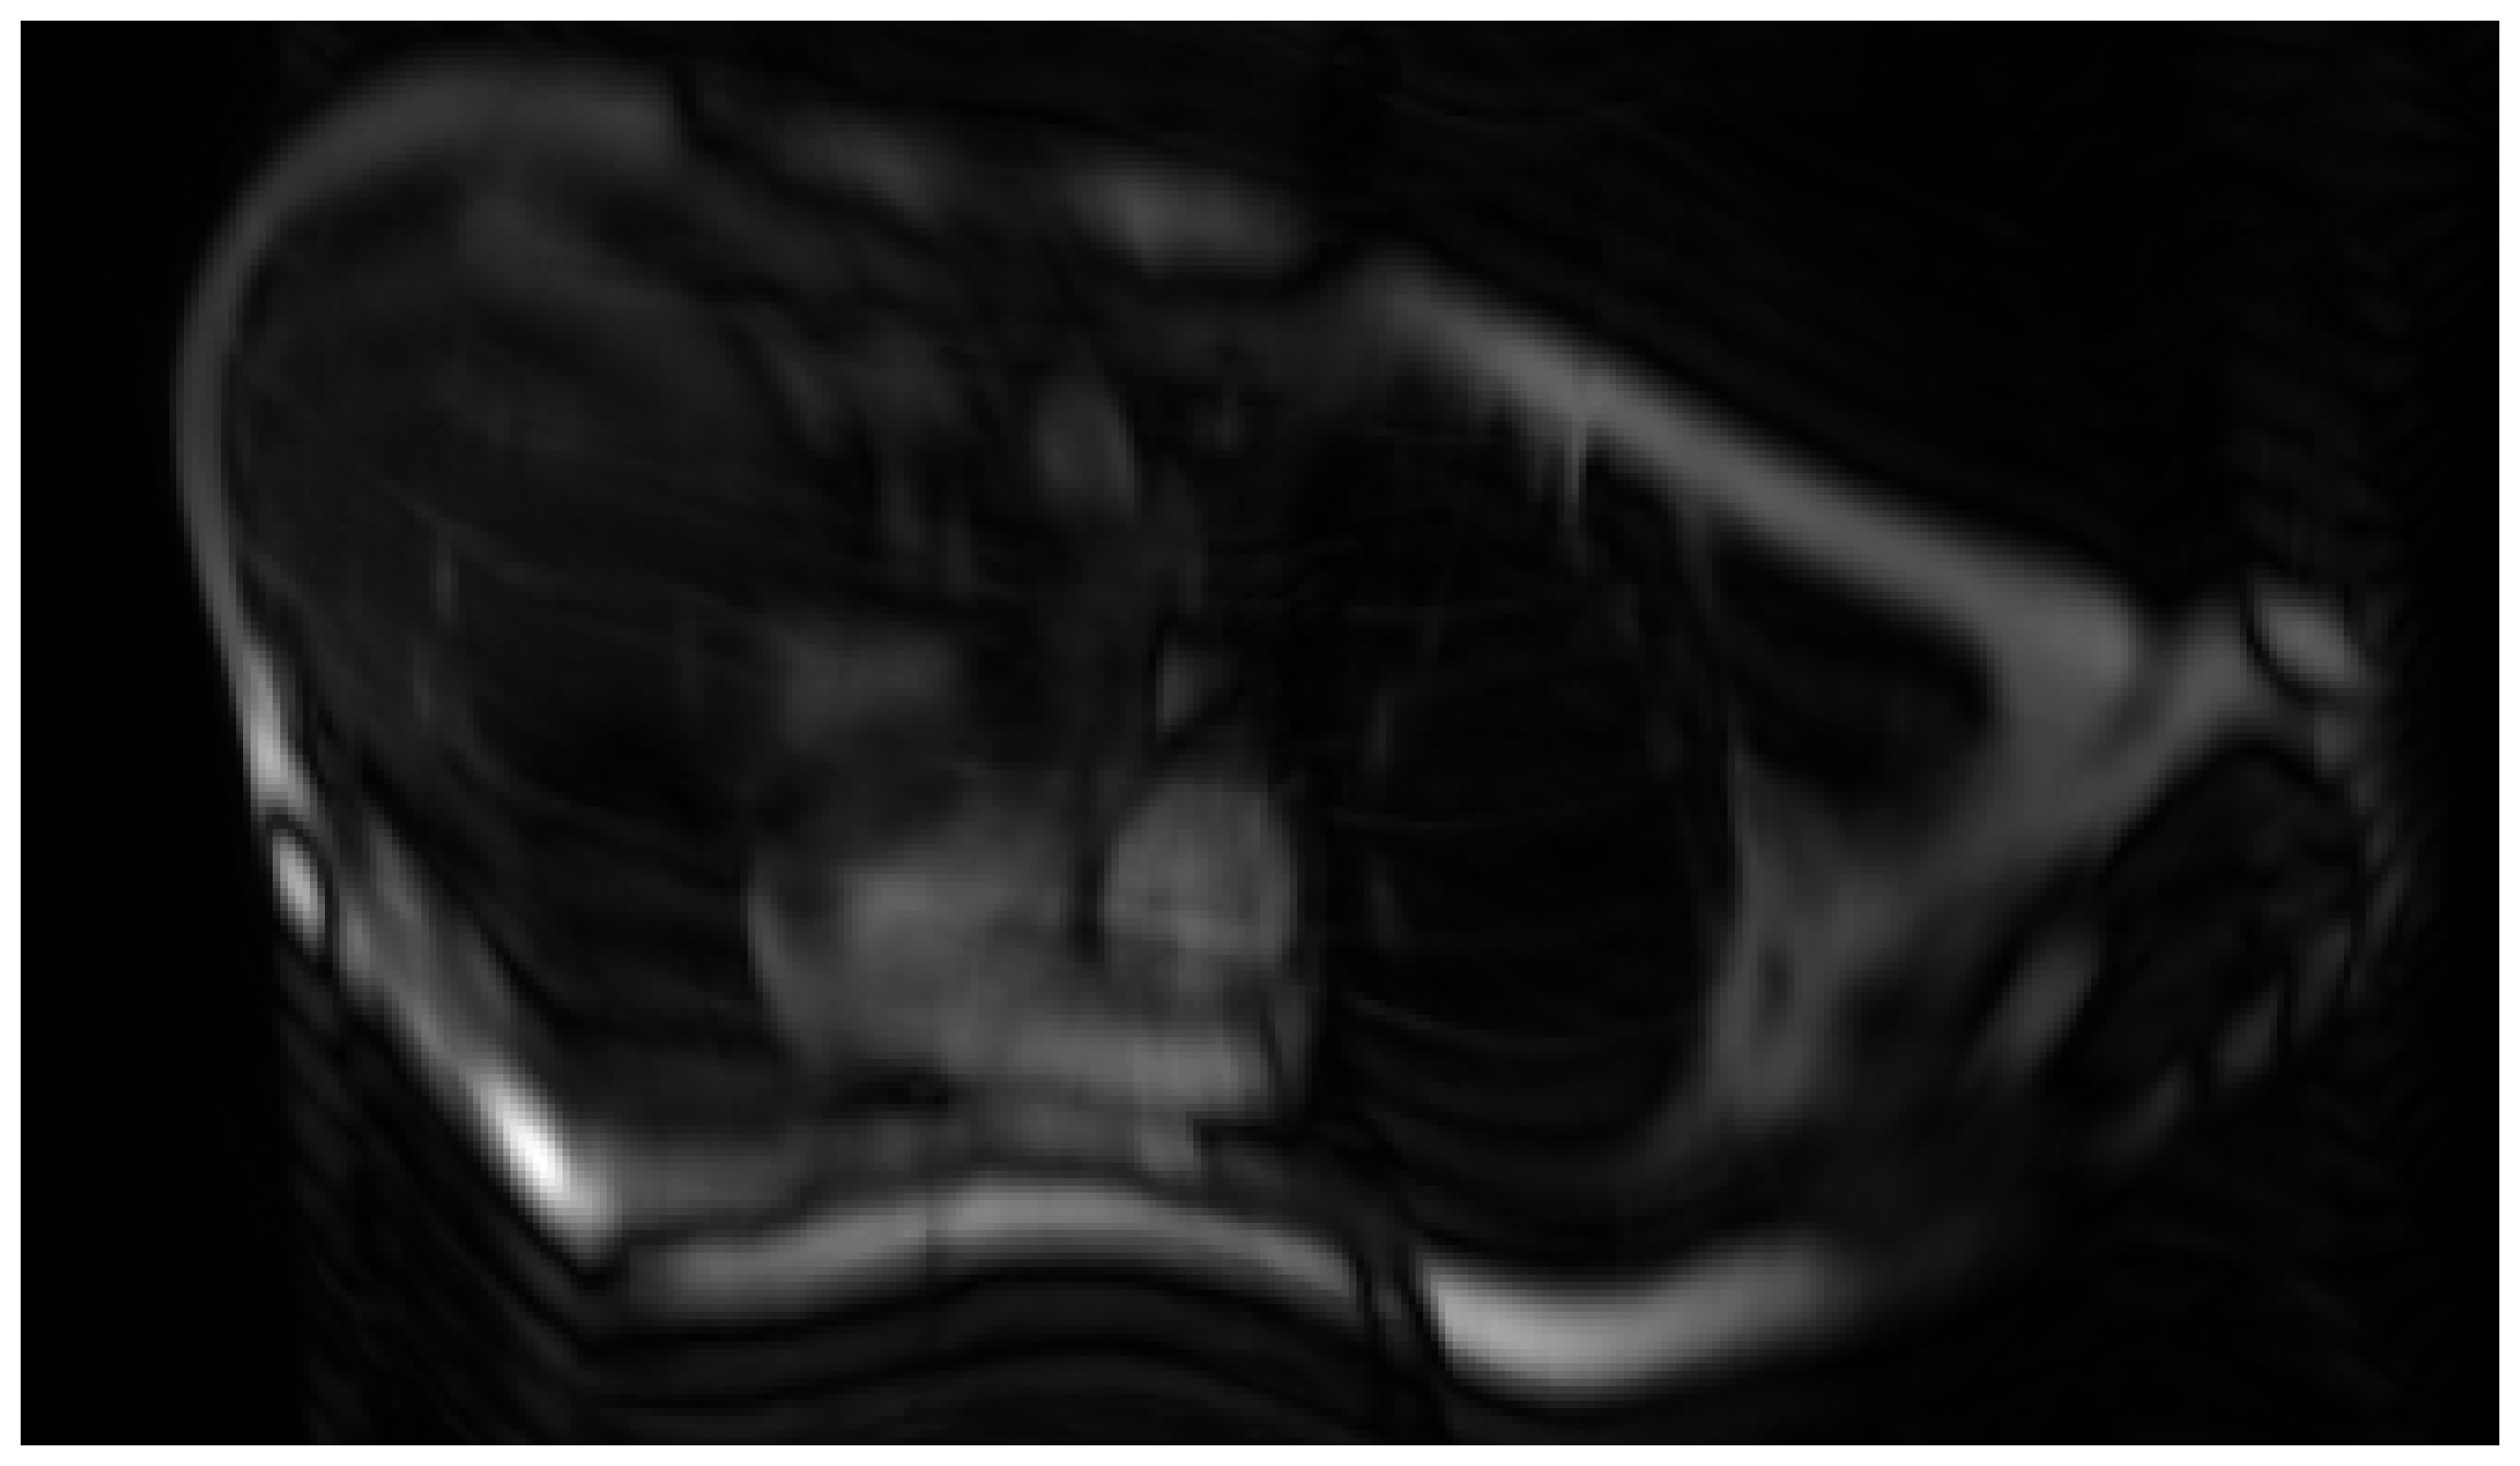
\includegraphics[width=\textwidth]{./Images/LungMotion2.png}
    		%\caption{Second subfigure.}
    		\label{fig:LungMotion2}
	\end{subfigure}
	\\
	\begin{subfigure}{0.475\textwidth}
    		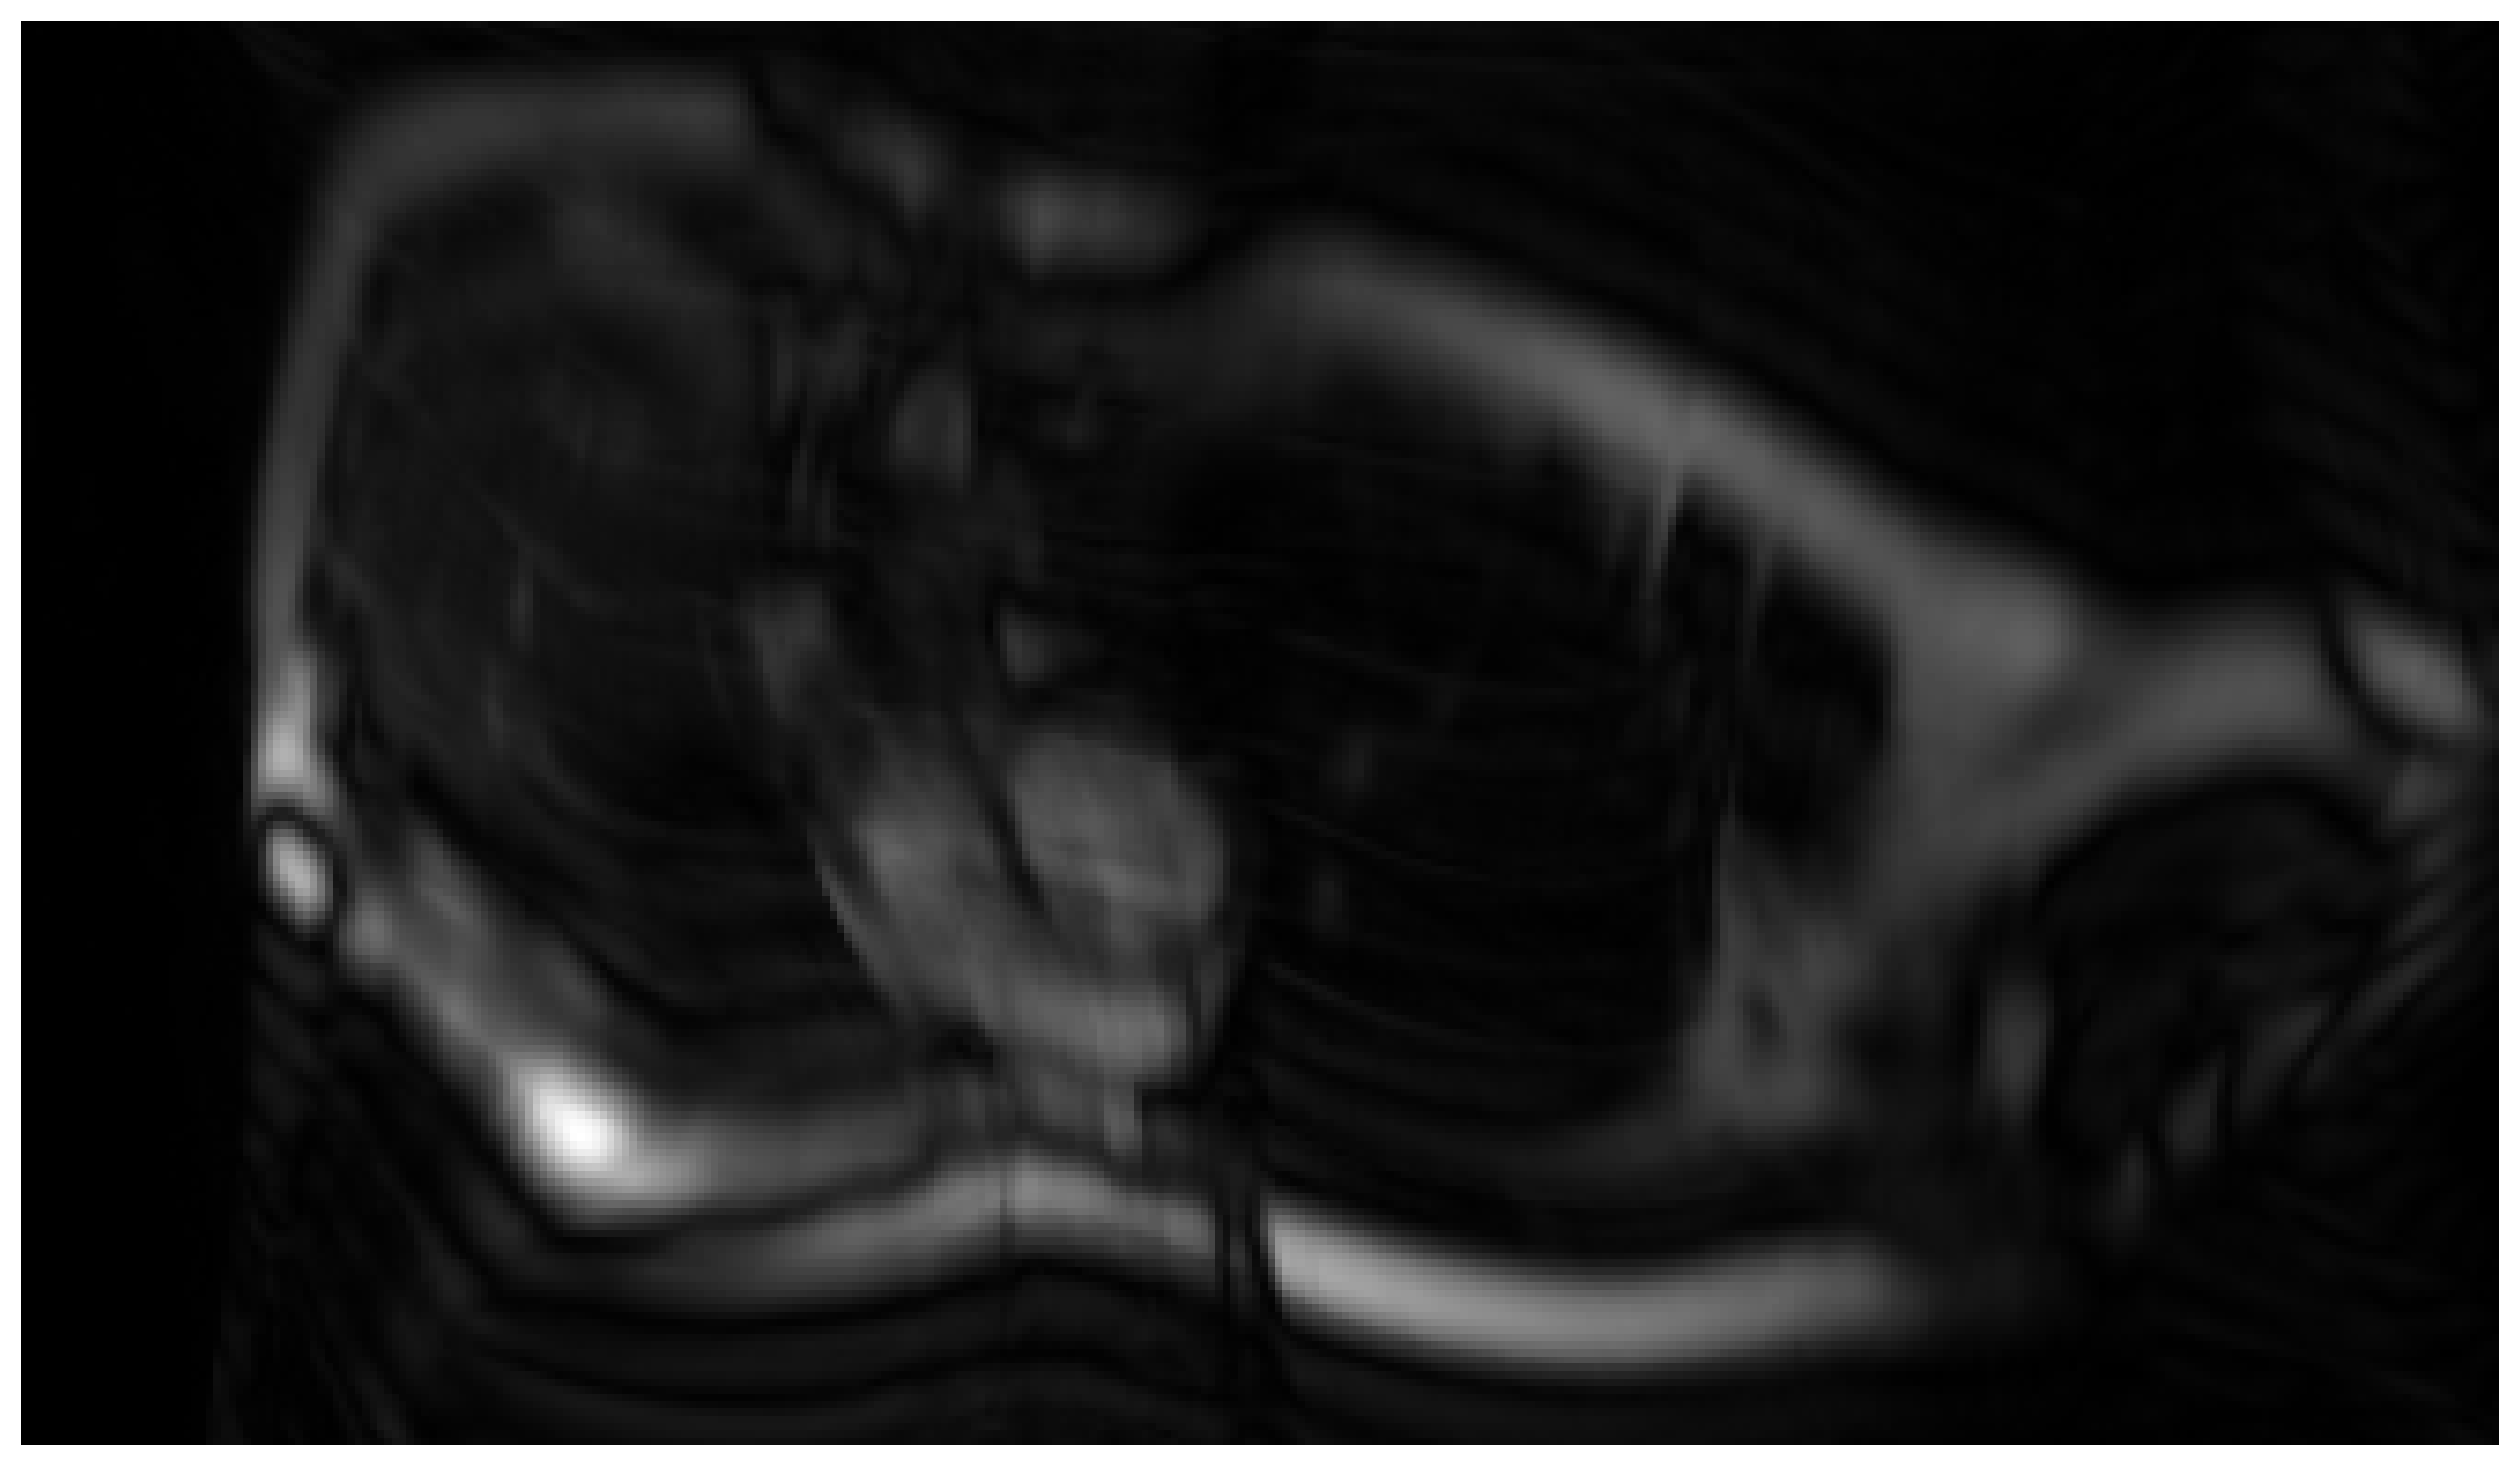
\includegraphics[width=\textwidth]{./Images/LungMotion3.png}
    		%\caption{First subfigure.}
    		\label{fig:LungMotion3}
	\end{subfigure}
	\hfill
	\begin{subfigure}{0.475\textwidth}
    		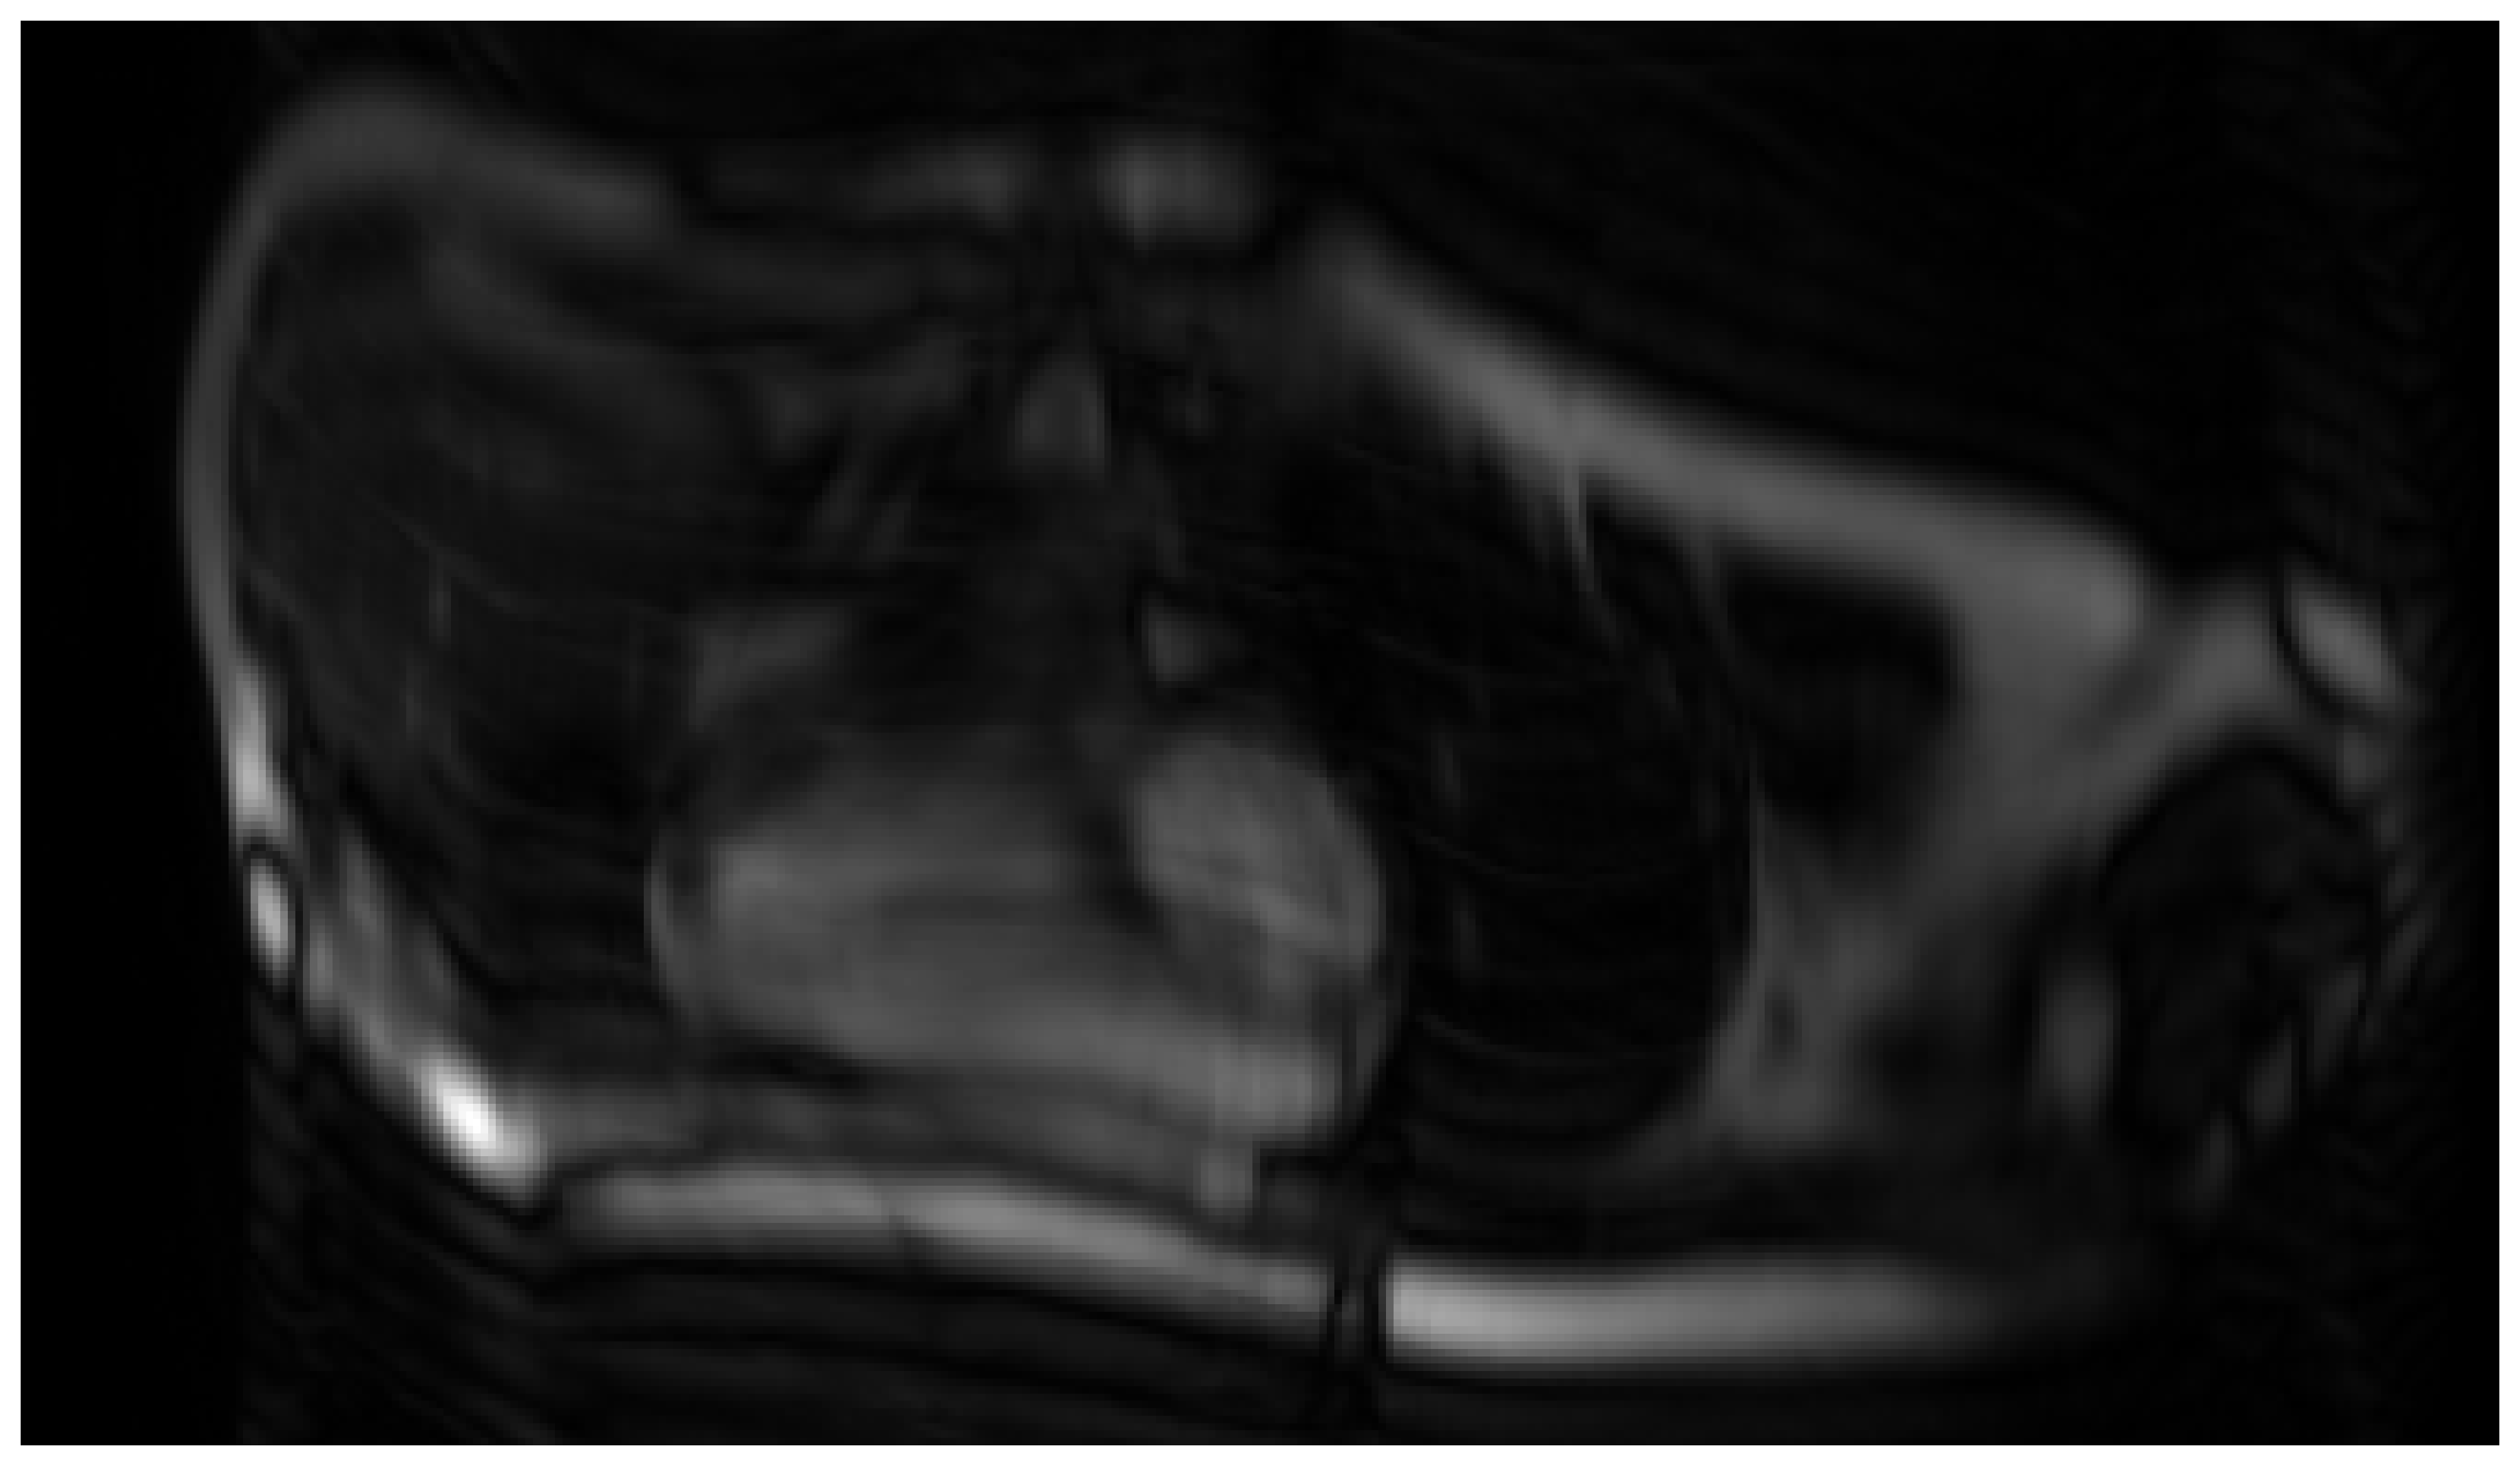
\includegraphics[width=\textwidth]{./Images/LungMotion4.png}
    		%\caption{Second subfigure.}
    		\label{fig:LungMotion4}
	\end{subfigure}
	\caption{$L=4$ images with simulated lung motion for the same cardiac frame (background was cropped out).}
	\label{fig:LungMotion}
\end{figure}


\section{Experiments} \label{Sec:Experiments}
In the following chapter the different experiments that were conducted are described and explained. 
%First was frame-to-frame registration on cardiac data from the \emph{CMRxRecon} dataset to lay the basis for later experiments with a motion-correcting reconstruction pipeline.
First, experiments were conducted on the \emph{ACDC} dataset to find the optimal parameters for our model using ground truth segmentations. Then a motion-compensated reconstruction pipeline was used as an down-stream task on the \emph{CMRxRecon} dataset.


\subsection{Ablation Studies and Parameter Tests} \label{SubSec:ParameterTestsACDC}
As the evaluation on the \emph{CMRxRecon} dataset is limited to image similarity measures, further testing was done on the \emph{ACDC} dataset which contains cardiac data with segmentations. These can be used to better evaluate the registration performance by using e.g. the Dice score. The tests include comparisons between \emph{Fourier-Net}, \emph{Fourier-Net+} and \emph{4xFourier-Net}, parameter tests for the starting channel size, FT crop size as well as comparisons with VoxelMorphs and dense versions of the three networks.


\subsubsection{Fourier-Net versus Fourier-Net+} \label{SubSubSec:Fourier-NetvsFourier-Net+}
First, \emph{Fourier-Net}, \emph{Fourier-Net+} and \emph{4xFourier-Net}, as introduced in sections~\ref{SubSec:Fourier-Net} and~\ref{SubSec:Fourier-Net}, are compared using both the baseline and diffeomorphic versions. Additionally, network versions creating dense instead of band-limited displacements were used for comparison. The registration performance was evaluated on the test set using the percentage of Dice scores calculated with and without the background label, percentage of SSIM, MSE multiplied by $10^{-3}$ (denoted by m for milli) and the percentage of negative Jacobian determinant of deformation. The mean inference time on the GPU together with memory consumption for each model are also added to the comparison with the latter containing number of trainable model parameters, mult-add operations (in millions or billion as denoted by M or G) and the total memory in Megabyte (MB). The latter is only given for the normal versions as the diffeomorphic version require the same amount of memory as well as the baseline dense versions. The first network was trained for a maximum of 15 epochs with early stopping activating after 3 epochs without improvement of the validation Dice score. The other variants were than trained with the same number of epochs, which worked out to be only 6 epochs due to the large training set in the experiments without any data augmentation. All networks were trained on the fully sampled \emph{ACDC} data with MSE as the unsupervised similarity loss, a channel size of 8, learning rate of 0.0001 and $\lambda=0.01$. \emph{Fourier-Net+} and \emph{4xFourier-Net} used a FT crop size of $48 \times 48$ for these experiments. All of these parameters were constant for the diffeomorphic and dense versions of the networks. The results and subsequent discussion can be found in section~\ref{SubSec:ResultsFourier-NetvsFourier-Net+ACDC}.


\subsubsection{Starting Channel Size} \label{SubSubSec:StartingChannelsACDC}
Next, the impact of the starting channels (see section~\ref{SubSec:Fourier-Net}) on the \emph{ACDC} data was examined as these dictate the number of features that the network uses. For this, \emph{Fourier-Net+} and \emph{4xFourier-Net+} was trained with MSE-loss, a learning rate of $0.0001$, $\lambda = 0.01$, FT crop of $48 \times 48$ and no diffeomorphic transform. The experiments were again only conducted on the fully sampled data. Four different channel sizes were used for training: $8$, $16$, $32$ and $64$. The first network variant was trained with early stopping, which ended at 6 epochs. For better comparability, the other network variants were also trained with the same number of epochs. The registration performance was evaluated on the test set using the percentage of the Dice score calculated once on all labels, once without the background using only the cardiac labels, as well as the SSIM in percent, MSE multiplied by $10^{-3}$ and the percentage of negative Jacobian determinant of deformation. Additionally the number of network parameters, number of mult-add operations (in millions or billion as denoted by M or G) and memory consumption in Megabyte (MB) are listed for all network variants to better compare the relationship between registration performance and memory consumption to potentially find a optimal configuration for both performance and efficiency. The mean inference time was measured on GPU in seconds. The results and subsequent discussion can be found in section~\ref{SubSec:ResultsStartingChannelsACDC}.


\subsubsection{Fourier-Transform Crop Size} \label{SubSubSec:FTCropSize}
The FT crop size, used for compressing the input images, is a parameter specific to \emph{Fourier-Net+} and \emph{4xFourier-Net+}. Four different sizes of the FT crop were analyzed: $80 \times 168$, $40 \times 84$, $48 \times 48$ and $24 \times 24$. A larger crop would obviously compress the images less, thus leading to less efficiency, however, a very small crop, while very efficient, might lose some of the image details leading to a decrease in performance. The experiments were again only conducted on the fully sampled data as one would expect similar results on subsampled data. The network variants were trained with MSE as the unsupervised similarity loss, a channel size of 8, learning rate of 0.0001 and $\lambda=0.01$. Again, the networks were trained for only 5 epochs, as this is were the first model ended training due to early stopping. The registration performance was evaluated on the test set using the Dice score calculated once on all labels, once without the background, as well as the SSIM, MSE and the percentage of negative Jacobian determinant of deformation. Additionally, the number of network parameters, number of mult-add operations in millions (M) and memory consumption in Megabyte (MB) are listed for all network variants to better compare the relationship between registration performance and memory consumption to potentially find a optimal configuration for both performance and efficiency. The mean inference time was measured on GPU in seconds. The results and subsequent discussion can be found in section~\ref{SubSec:ResultsFTCropSize}.


\subsubsection{Comparison with VoxelMorph} \label{SubSubSec:ComparisonVoxelMorph}
After finding parameters which optimize registration performance while trying to minimize memory consumption, a comparison to another commonly used registration network should be made. For this, a diffeomorphic version~\cite{VoxelMorphDiff} of the well known \emph{VoxelMorph}~\cite{Voxelmorph} was used with integration steps $T=7$. It was trained with the default number of layers, MSE as the similarity loss, a learning rate of 0.0001, $\lambda=0.01$. It provides a dense displacement field to align the image pair. For comparison \emph{Fourier-Net}, \emph{Fourier-Net+} and \emph{4xFourier-Net+} were trained for 6 epochs with MSE as the unsupervised similarity loss, a channel size of 16, learning rate of 0.0001 and $\lambda=0.01$ as well as a FT crop size of $48 \times 48$, which provide a good balance of performance and memory imprint for the networks. To evaluate registration performance, the Dice score was again computed for all labels and without the background as well as the similarity metrics SSIM, MSE and the percentage of negative Jacobian determinant of deformation. All networks were trained on the fully sampled \emph{ACDC} data. The inference times of all networks were computed on the GPU and the number of network parameters, number of mult-add operations in billions (G) and memory consumption in Megabyte (MB) are also given to further compare the efficiency of the networks. The results can be seen in section~\ref{SubSec:ResultsComparisonVoxelMorph}.


\subsubsection{Dense Displacement on Accelerated Data} \label{SubSubSec:DenseDisplacementAcc}
The difference between a dense displacement field and a band-limited one was already explored in a previous section, but only on fully sampled, not accelerated data. This section explores potential performance changes on the latter with the hypothesis that the network variants with the dense displacement will perform worse than the variants with the band-limited displacement field for strongly subsampled data. This expectation stems from the fact that frequencies outside the center region of the k-space are dropped for the accelerated data thus reducing the advantage of the dense displacement in comparison to the band-limited (i.e. center-cropped) displacement. \\
The tests again included \emph{Fourier-Net}, \emph{Fourier-Net+} and \emph{4xFourier-Net+}, which were all trained for 6 epochs with MSE as the unsupervised similarity loss, a channel size of 16, $48 \times 48$ FT crop, learning rate of 0.0001 and $\lambda=0.01$. The registration performance was evaluated on the test set using the Dice score calculated once on all labels, once without the background, as well as the SSIM, MSE and the percentage of negative Jacobian determinant of deformation. Additionally, the number of network parameters, number of mult-add operations in millions (M) and memory consumption in Megabyte (MB) are given.

\subsection{Registration Performance on Subsampled Data} \label{SubSubSec:ComparisonSubsampling}
After comparing \emph{Fourier-Net}, \emph{Fourier-Net+} and \emph{4xFourier-Net+} with both dense and band-limited displacement fields as well as another comparison with \emph{VoxelMorph} on fully sampled data 
%to access the difference in registration performance and memory consumption 
an extension to subsampled data needs to be made. For this \emph{Fourier-Net}, \emph{Fourier-Net+} and \emph{4xFourier-Net+} were compared to a baseline consisting of the unaligned test image pairs as well as \emph{NiftyReg}~\cite{NiftiReg}, \emph{VoxelMorph}~\cite{Voxelmorph} and \emph{LAPNet}~\cite{LAPNet}. Thus, observations of the performance on accelerated data can be made as well as comparisons to the aligned baseline (which all methods should aim to beat), a traditional registration algorithm, a dense registration network working in the image domain and a another dense network which works in the k-space domain.\\
\emph{Fourier-Net}, \emph{Fourier-Net+} and \emph{4xFourier-Net+} were trained for 6 epochs with MSE as the unsupervised similarity loss, a channel size of 16, learning rate of 0.0001 and $\lambda=0.01$ as well as a FT crop size of $48 \times 48$ for all subsampling data. VoxelMorph was trained with default layers and MSE as the similarity loss, a learning rate of 0.0001 and $\lambda=0.01$. Three different acceleration factors were tested: $R=4$, $R=8$ and $R=10$. For reference, the data for the fully sampled data ($R=0$) is also provided. The registration performance of all methods was evaluated on the test set using the Dice score calculated once on all labels, once without the background, as well as the SSIM and MSE as image metrics. All times are computed on CPU for better comparability as \emph{NiftyReg} currently only works on CPU as the GPU capable versions were deprecated and the other networks would gain an unfair time advantage when ran on GPU. The baseline obviously has no time associated as it only denotes the metrics on the test data before registration. The results and an comprehensive discussion are provided in section~\ref{SubSec:ResultsComparisonSubsampling}.


\subsection{Motion-Compensated Reconstruction Pipeline} \label{SubSec:IntegrationMotion-CompensatedReconstructionPipeline}
After multiple parameter tests and ablation studies to find optimal network parameters, a down-stream experiment is conducted to show the usability of the networks in real-world applications. For this a motion-compensated reconstruction pipeline was chosen where the network can be used to correct the motion-corrupted data. As the \emph{ACDC} dataset only contains already reconstructed data, the next tests were all conducted on the \emph{CMRxRecon} dataset. Thus, the domain gap between the datasets is assessed first before the experiments using the reconstruction pipeline are described.

\subsubsection{Domain Translation} \label{SubSubSec:DomainTranslation}
As the following experiments need to be conducted on the \emph{CMRxRecon} dataset as it provides k-space data and subsampling masks, the domain translation capabilities of \emph{Fourier-Net}, \emph{Fourier-Net+} and \emph{4xFourier-Net+} have to be tested before evaluating the reconstruction pipeline. For this the three networks, previously trained on \emph{ACDC}, were trained again from scratch on \emph{CMRxRecon}. They were then compared on the \emph{CMRxRecon} test data to see how similar the performance would be as the cardiac scans of the two datasets are fairly similar. The network parameter used (MSE-loss, 16 channels, $48 \times 48$ FT crop, learning rate 0.0001, $\lambda=0.01$) were the same for all network, however the networks were trained for 6 epochs on \emph{ACDC} and 14 epochs on \emph{CMRxRecon} as the latter has less training data. For evaluation again SSIM and MSE were used as image similarity metric. Note that the Dice score cannot be calculated as the \emph{CMRxRecon} dataset does not include segmentations for multi-coil data. Additionally, the percentage of negative Jacobian determinant of deformation and the inference time on GPU are given.


\subsubsection{Reconstruction Performance on Motion-Corrupted Data} \label{SubSubSec:ReconstructionPipeline}
As discussed in section~\ref{SubSec:Motion-CompensatedReconstruction}, neural networks can be used in motion-compensated MRI reconstruction pipelines for either the reconstruction or the corrected of motion between the frames. As \emph{Fourier-Net}, \emph{Fourier-Net+} and \emph{4xFourier-Net+} were already trained for frame-to-frame registration, they could be easily used for the latter. ESPIRiT~\cite{ESPIRiT} was used to simulate the coil sensitivity maps needed for a SENSE-type reconstruction from the provided k-space data using an eigenvalue decomposition~\cite{ESPIRiT}. For the SENSE~\cite{SENSE1} reconstruction, an iterative conjugate gradient algorithm was used as it is very memory effective due to \emph{Fourier-Net+} being a very small network and the fact that no big network is needed for the actual reconstruction as a lightweight algorithm does the work. \\ 
Two experiments were conducted on the \emph{CMRxRecon} dataset as it provides the needed k-space data (both fully sampled and accelerated) as well as the subsampling masks required for reconstruction. However, the cardiac scans only show a small amount of movement between frames due to cardiac movement no larger movement of e.g. the lung. Thus, the input images were further motion-corrupted as the cardiac motion present was deemed not severe enough. This process is detailed in section~\ref{SubSec:SimulatedMotion}. An overview of this augmentation incorporated into the reconstruction pipeline can be seen in Figure~\ref{fig:GeneralReconstructionPipeline}.\\
\emph{Fourier-Net}, \emph{Fourier-Net+} and \emph{4xFourier-Net+} have been pre-trained on image reconstructed from this data via an iFT for frame-to-frame registration using the optimal settings obtained in section~\ref{SubSec:ParameterTestsACDC} (MSE-loss, 16 channels, $48 \times 48$ FT crop, learning rate 0.0001, $\lambda=0.01$). As the \emph{CMRxRecon} dataset does not include segmentations for Dice calculation, image similarity metrics need to be utilized. For this, SSIM and MSE were used again, however, the PSNR (see section~\ref{SubSec:NetworkTrainingAndTesting}) and HaarPSI~\cite{HaarPSI} were also added. For comparison \emph{VoxelMorph} was used. The results can be seen in section~\ref{SubSec:ResultsReconstructionPipeline}.


% general reconstruction pipeline with synthetic motion-corrupted 
\begin{figure}[h] %tpb
	\centering
	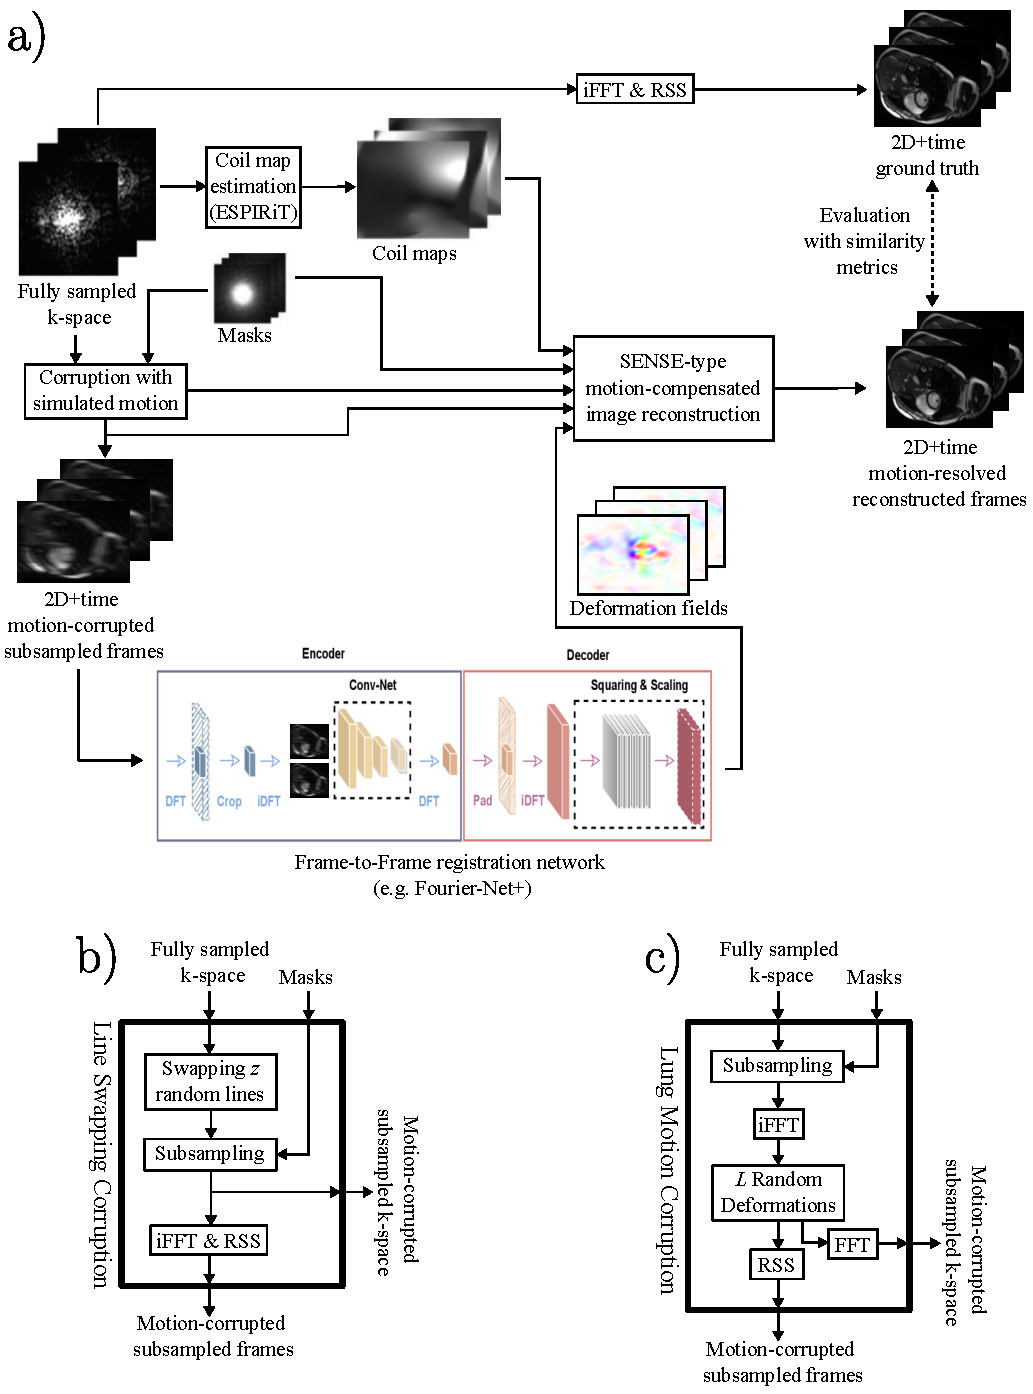
\includegraphics[width=\linewidth]{./Images/GeneralReconstructionPipeline.pdf} 
	\caption{Overview of the generalized reconstruction pipeline in a) using \emph{Fourier-Net+} as a registration network (Figure inspired by~\cite{Kuestner2022}). The k-space data is corrupted with synthetic motion, either through swapping $z$ random line (steps shown in b) or by via $L$ random deformation frames to simulate lung motion (shown in c)).}
	\label{fig:GeneralReconstructionPipeline}
\end{figure}
